% ------------------------------------------------
%
%論文內容次序:
% 1.考試合格證明
% 2.中英文摘要(論文以中文撰寫者須附英文延伸摘要)
% 3.誌謝
% 4.目錄
% 5.表目錄
% 6.圖目錄
% 7.符號
% 8.主文
% 9.參考文獻
% 10.附錄
%
% 註: 參考文獻書寫注意事項:
% (1).
%    文學院之中文文獻依分類及年代順序排列。
%    其他學院所之文獻依英文姓氏第一個字母
%    (或中文姓氏第一個字筆劃)及年代順序排列。
%
% (2).
%    期刊文獻之書寫依序為:
%        姓名、文章名稱、期刊名、卷別、期別、頁別、年代。
%
% (3).
%    書寫之文獻依序為:
%        姓名、書名、出版商名、出版地、頁別、年代。
%
% ------------------------------------------------

% 封面內頁 Inner Cover
%
% 封面: 顯示所有封面內容, 但沒有學校Logo)
%     主要用在印刷版, 如精裝版 或 平裝版
%     (使用cover.tex來產生)
%
% 內頁: 顯示所有封面內容, 但有學校Logo
%     主要用在電子版 + 印刷版
%
% 只要是印刷版, 不論是精裝版或平裝版, 都是 封面 (殼/皮) + 內頁.
% 只有在電子版時, 第一頁就是封面內頁.

\DisplayInnerCover

% ------------------------------------------------

% 口試証明文件
\DisplayOral

% ------------------------------------------------

% 摘要 Abstract
% 除了外籍生, 本地生和僑生都是要編寫中文和英文摘要
% 論文以中文撰寫須以英文補寫 800 至 1200 字數的英文延伸摘要 (Extended Abstract)
% 詳細可看附件的學校要求或看example中的英文延伸摘要

% ------------------------------------------------
\StartAbstractChi
% ------------------------------------------------

這是國立成功大學碩博士用畢業論文的LaTex模版. 這模版是使用學校最新的畢業論文要求來設計(參考: 附錄 - 撰寫論文須知 P.\RefPage{appendix:thesis-spec}).

這模版的目標是為了提供學生可以使用LaTex來寫畢業論文. 但是各系所有各自的格式, 故請在使用前先留意自己的系所有沒有格式要求 (參考: 附錄 - 可使用的系所 P.\RefPage{appendix:acceptable-dept}). 如果沒有, 則這模版應該用來使用; 否則要看系所上的格式, 是否跟這模版有相同的寫法.

這模版的內容是我參考了我所拿到的一些畢業論文的LaTex模版設計, 跟系上老師的一些對話, 和上課所聽得出的結論和想法而寫出的, 所以某些地方會帶有我們濃郁的資工系味道. 另外如果有任何的老師 (不論本系外系)可以提供一些意見或想法的話, 我會十分感謝的.

這模版盡量以全自動化方式去處理一些不用你去煩惱的部份, 如排版和設計. 只留下要你去填寫的部份, 所以只要選擇和填入你的內容, 就能得到一份符合學校要求的畢業論文.

最後, 希望你使用愉快.

% ------------------------------------------------
% 如果在conf.tex中的\SetAbstractChiKeywords有設定任何的關鍵字,
% 那中文版的關鍵字會在使用\EndAbstractChi後同時顯示出來.
\EndAbstractChi
% ------------------------------------------------
             % 中文版
% ------------------------------------------------
\StartAbstract
% ------------------------------------------------

Write your abstract here.

Enjoy this templete.

% ------------------------------------------------
\EndAbstract
% ------------------------------------------------
             % 英文版
% ------------------------------------------------
\StartExtendedAbstract
% ------------------------------------------------

\ExtAbstractSummary{
The summary is a short, informative abstract of no more than 250 words. References should not be cited. The summary should (1) state the scope and objectives of the research, (2) describe the methods used, (3) summarize the results, and (4) state the principal conclusions. Text of the summary should be 12 pt Times New Roman font, single-spaced and justified. A single line space should be left below the title 'SUMMARY'. Leave a single line space above the key words listed below.
} % End of \ExtAbstractSummary{}

% ------------------------------------------------
\ExtAbstractChapter{INTRODUCTION}{
The purpose of the introduction is to tell readers why they should want to read your thesis/ dissertation. This section should provide sufficient background information to allow readers to understand and evaluate the paper's results.

The introduction should (1) present the nature and scope of the problem, (2) review related literature, (3) describe the materials used and method(s) of the study, and (4) describe the main results of the study.

All text in the main body of the extended abstract should be 12 pt Times New Roman font, single-spaced and justified. Main headings are placed in the centre of the column, in capital letters using 12 pt Times New Roman Bold font. Subheadings are placed on the left margin of the column and are typed in 12 pt Times New Roman Bold font.
} % End of \ExtAbstractChapter{}

% ------------------------------------------------
\ExtAbstractChapter{MATERIALS AND METHODS}{
There is flexibility as to the naming of the section (or sections) that provide information on the method(s) or theories employed. The methodology employed inthe work must be described in sufficient detail or with sufficient references so that the results could be duplicated.

Your materials should be organised carefully. Include all the data necessary to support your conclusions, but exclude redundant or unnecessary data.
} % End of \ExtAbstractChapter{}

% ------------------------------------------------
\ExtAbstractChapter{RESULTS AND DISCUSSION}{
The results and discussion sections present your research findings and your analysis of those findings. The results of experiments can be presented as tables or figures.
} % End of \ExtAbstractChapter{}

% ------------------------------------------------
\ExtAbstractSection{Figures and Tables}{
Figures may be integrated within the results section of the extended abstract, or they can be appended to the end of the written text. Figures should be black \& white. They should be no wider than the width of the A4 page.

Tables can be created within Word. As noted for figures above, if a table is to be placed within the text, it can be no wider than the width of the A4 page. Larger tables will need to be placed at the end of the abstract.

Figures and tables should be numbered according to the order they are referenced in the paper. Figures and tables should be referred to by their number in the text. When referring to figures and tables in the text, spell out and capitalize the word Figure or Table. All figures and tables must have captions.
} % End of \ExtAbstractSection{}

% ------------------------------------------------
\ExtAbstractSection{Captions}{
Captions should clearly explain the significance of the figure or table without reference to the text. Details in captions should not be restated in the text. Parameters in figure captions should be included and presented in words rather than symbols.

Captions should be placed directly above the relevant table and beneath the relevant figure. The caption should be typed in 12 pt Times New Roman Bold font. Spell out the word 'Table' or 'Figure' in full. An example table and a figure follow.
} % End of \ExtAbstractSection{}

% ------------------------------------------------
\InsertImage
  [scale=0.5, align=center,
    caption={Specifications of the engine}]
  {./example/abstract/pic/extended-abstract-1.jpg}

\InsertImage
  [scale=0.5, align=center,
    caption={HC emission as a function of equivalence ratio}]
  {./example/abstract/pic/extended-abstract-2.jpg}
% ------------------------------------------------

\ExtAbstractChapter{CONCLUSION}{
This section should include (1) the main points of your paper and why they are significant, (2) any exceptions to, problems with, or limitations to your argument, (3) agreements or disagreements with previously published work, (4) theoretical and practical implications of the work, and (5) conclusions drawn.
} % End of \ExtAbstractChapter{}

% ------------------------------------------------
\EndExtendedAbstract
% ------------------------------------------------
        % 英文延伸摘要

% ------------------------------------------------

% 誌謝 Acknowledgments
% 誌謝正常應該只要寫一種版本就可,
% 提供2種以自行選擇所顯示的語言.
% 2種同時編寫都是可以的.

% ------------------------------------------------
\StartAbstractChi
% ------------------------------------------------

這是國立成功大學碩博士用畢業論文的LaTex模版. 這模版是使用學校最新的畢業論文要求來設計(參考: 附錄 - 撰寫論文須知 P.\RefPage{appendix:thesis-spec}).

這模版的目標是為了提供學生可以使用LaTex來寫畢業論文. 但是各系所有各自的格式, 故請在使用前先留意自己的系所有沒有格式要求 (參考: 附錄 - 可使用的系所 P.\RefPage{appendix:acceptable-dept}). 如果沒有, 則這模版應該用來使用; 否則要看系所上的格式, 是否跟這模版有相同的寫法.

這模版的內容是我參考了我所拿到的一些畢業論文的LaTex模版設計, 跟系上老師的一些對話, 和上課所聽得出的結論和想法而寫出的, 所以某些地方會帶有我們濃郁的資工系味道. 另外如果有任何的老師 (不論本系外系)可以提供一些意見或想法的話, 我會十分感謝的.

這模版盡量以全自動化方式去處理一些不用你去煩惱的部份, 如排版和設計. 只留下要你去填寫的部份, 所以只要選擇和填入你的內容, 就能得到一份符合學校要求的畢業論文.

最後, 希望你使用愉快.

% ------------------------------------------------
% 如果在conf.tex中的\SetAbstractChiKeywords有設定任何的關鍵字,
% 那中文版的關鍵字會在使用\EndAbstractChi後同時顯示出來.
\EndAbstractChi
% ------------------------------------------------
             % 中文版
% ------------------------------------------------
\StartAbstract
% ------------------------------------------------

Write your abstract here.

Enjoy this templete.

% ------------------------------------------------
\EndAbstract
% ------------------------------------------------
             % 英文版

% ------------------------------------------------

% 目錄 (內容, 圖表和圖片) Index of contents, tables and figures.
% 內容會自動產生 The indices will generate in automate.
\DisplayIndex                 % 顯示索引
\DisplayTablesIndex   % 顯示表格索引
\DisplayFiguresIndex  % 顯示圖片索引

% ------------------------------------------------

% Nomenclature
% ------------------------------------------------
\StartSection{術語 Nomenclature}{chapter:how-to:write:nomenclature}
% ------------------------------------------------

Nomenclature在定義一些在整份論文中所會用到的變數是很常用到的. 它的位置會出現在文章當中或是在Chapter 1之前. 它的設計沒有一個標準答案, 在不同的情況下可能有不同顯示方式, 但它基本上跟一張Table是沒差的. 而它在Latex中是使用一個package名為`nomencl'.\\

但經過研究了一下package `nomencl'或tabbing這些用來建Nomenclature的方式後, 發現`nomencl'在設計上反而會增加在產生論文時的步驟; 而tabbing要自行定義一個闊度才能弄得比較好看, 但同時內容卻出現沒法置中和設計上等一些問題. 故最後決定直接套用Table來讓同學更能自由的設計不同的Nomenclature table.\\

設計Nomenclature table需要2個知識或工具:\\
1) 設計一張Table, 這邊請參考P. \RefPage{chapter:how-to:write:table}.\\
2) 有關所需要用到的符號, 請參考Equation (P. \RefPage{chapter:how-to:write:equation})中所使用到的工具, Texmarker左邊的工具列, 或看這幾個網頁\RefBib{web:symbols:site1}\RefBib{web:symbols:site2}\RefBib{web:symbols:site3}, 應該已經足夠同學們寫出合適的符號.

% ------------------------------------------------
%\newpage
\StartSubSection{使用方式}

如果是指是在Chapter 1之前的一大張的Nomenclature table, 為Nomenclature Chapter. 
  \begin{verbatim}
  \StartNomChapter{ NAME }{ LABEL }
  \EndNomChapter
  \end{verbatim}
Nomenclature Chapter跟一般Chapter的使用方式是一樣的, 但差別在於不會出現`Chapter'這字眼. 而由於大家的Nomenclature Chapter name可能不一樣, 故跟Chapter一樣可設定自行的name.\\

而如果是在文章當中的Nomenclature table. 基本上就是使用同一個的`\verb|\InsertTable|', 但還可以使用`nomtitle'來設定標題. `nomtitle'跟`caption'的差別是, 使用`nomtitle'所顯示出來的標題是沒有`Table XX:'為開頭, 同樣都是使用`pos'來控制題目的位置.

  \EmptyLine
  \begin{DescriptionFrame}
  \begin{verbatim}
  Options 設定
    nomtitle:   Nomenclature 標題 (選填)
    ...

  E.g
    \InsertTable
    [nomtitle={這是Nomenclature Table的標題}]
      {
        ...
      }
  \end{verbatim}
  \end{DescriptionFrame}
  \EmptyLine

有關這個的用法可參考`example/nomenclature/nomenclature.tex'中的Nomenclature Chapter所demo的例子, 那2個例子只是最簡單的Nomenclature table設計, 應該足夠同學們去弄出合適自己的Nomenclature table的設計.



% ------------------------------------------------

% Introduction section
% ------------------------------------------------
\StartChapter{Introduction}{chapter:introduction}
% ------------------------------------------------

\StartSection{介紹}

這是國立成功大學碩博士用畢業論文的LaTex模板. 本模板是使用學校最新的畢業論文要求來設計(參考: 附錄 - 撰寫論文須知 P.\RefPage{appendix:thesis-spec}).

雖然本模板的目標是為了提供學生可以使用LaTex來寫畢業論文. 但是各系所有各自的格式, 所以做了一個表列出已知的系所情況(參考: 附錄 - 可使用的系所 P.\RefPage{appendix:acceptable-dept}), 故請在使用前先留意自己的系所有沒有格式要求. 如果沒有, 則本模板應該是可以用來使用; 否則要看系所上的格式, 是否跟本模板有相同的寫法.

本模板分以下幾個主要部份來進行教學:
\begin{enumerate}
  \item 本模板的架構設計
  \item 設定本模板的一些資料以轉成你的論文
  \item 介紹Latex和本模板所提供的語法
  \item 最後有一個chapter為"老師們的話"(Chap. \RefTo{chapter:words-from-teacher})寫了一些老師對論文的想法和意見, 以供同學們留意
\end{enumerate}
同學們只要閱讀完後, 把部份的檔案直接copy和修改內容, 應該很快就能上手本模板去寫自己的論文.

另外在附錄(appendix)附上了一些重要的學校的文件, 由於本模板很接近完善, 故直接使用本模板後可不需再閱過學校相關規定之文件, 所以該類文件置於此僅為備考用.

% ------------------------------------------------
%\newpage

\begin{description}
  \item[版權 License] \hfill
  \InsertImage
    [scale=0.8, align=center,
      caption={CC Attribution-NonCommercial-ShareAlike License},
      label={fig:appendix:by-nc}]
    {./example/introduction/pic/by-nc-sa.png}

    本著作(ncku-thesis-templete-latex\RefBib{web:this-project:github})採用創用 CC 姓名標示-非商業性-相同方式分享 4.0 授權條款.

    This work(ncku-thesis-templete-latex\RefBib{web:this-project:github}) is licensed under Creative Commons Attribution-NonCommercial-ShareAlike 4.0 International License.

  詳細請看'LICENSE'這檔案中的條款說明.

  \item[版本修改 ChangeLog] \hfill
    % ------------------------------------------------
\begin{description}
  \item[v1.3.0] 重大改版 (如果是使用升級方式, 請注意以下所修改的部份有沒有影響自身的版本)\hfill
    \begin{description}
      \item[其他] \hfill
        \begin{enumerate}
          \item 更新CONTRIBUTE中的名單和使用的稱號
        \end{enumerate}
    \end{description}

  \item[v1.2.8] 修正日期在英文書脊中, 會因月份文字的長度而影響位置不一樣的問題

  \item[v1.2.7] \hfill
    \begin{enumerate}
      \item 增加可放置論文題目的長度. 修正在封面和Oral文件的樣板中, 會在題目沒有很長情況下, 被強迫斷行. 長度控制交由同學自己斷行, 以造出比較漂亮題目
      \item 修正書脊中題目跟學位不是同一個高度的問題
      \item 修正英文Oral文件的樣板會出現頁碼的問題
    \end{enumerate}

  \item[v1.2.5] 修正在'Objective'和'Acknowledgments'的錯誤內容

  \item[v1.2.4] 增加英文封面可同時顯示中英文 (\href{https://github.com/wengan-li/ncku-thesis-templete-latex/issues/3}{Issue \#3})

  \item[v1.2.3] \hfill
    \begin{enumerate}
      \item 修正統一使用'Fig'去取代'Fig.', 因為當使用'Fig.'時會產生更大的空格
      \item 修正在'表格 Table'中的圖片位置
      \item 移除在'圖片 Image'的'多張'中舊API的說明文字
      \item 修正在'圖片 Image'中插入多張的圖片時, 不管是主圖或子圖片都推薦使用'align = center'來進行置中, 除非是為了特殊的原因
    \end{enumerate}

  \item[v1.2.2] 修正在'Induection'中的'ChangeLog'和'License'中一些奇怪多餘的空白

  \item[v1.2.1] 修正中文書脊文字位置錯誤問題

  \item[v1.2.0] \hfill
    \begin{enumerate}
      \item Appendix新增'常見問題Q\&A'
      \item 把'Induection'中的'ChangeLog'改使用為單一'.tex'檔去存放
      \item 增加字眼'共同指導'或'Co-advisor'在封面上 (\href{https://github.com/wengan-li/ncku-thesis-templete-latex/issues/2}{Issue \#2})
      \item 重新調整中文封面中的中英文名字2邊的中間空間的大小, 以防止中文名字有4個字時, 出現overlap的問題
    \end{enumerate}

  \item[v1.1.6] 刪除'Induection'和'README.md'中的'版本 Version'

  \item[v1.1.5] 修正每個Chapter的第一頁的頁碼位置跟其他頁面不同的問題 (\href{https://github.com/wengan-li/ncku-thesis-templete-latex/issues/1}{Issue \#1})

  \item[v1.1.4] 修正目錄自己沒有在目錄的Linking中出現

  \item[v1.1.3] 修正README.md中內容的位置錯誤

  \item[v1.1.2] \hfill
    \begin{enumerate}
      \item 重寫有關figure API的code, 增加和優化那些功能 (如增加align)
      \item 更新README.md的內容
      \item 增加ChangeLog
    \end{enumerate}

  \item[v1.1.1] \hfill
    \begin{enumerate}
      \item 把'Abstract'的中文版本是以'摘要'來顯示
      \item 修改和改良有關oral文件的一些path位置
    \end{enumerate}

  \item[v1.1.0] \hfill
    \begin{enumerate}
      \item 增加版權資料到一些核心檔案
      \item 修改和增加一些圖書館要求的內容
      \item 修改有關abstract的一些path位置
      \item 正式得到學校有關部門對這模板的接受
    \end{enumerate}

  \item[v1.0.1] 修改少量錯誤的內容和URL連接

  \item[<= v1.0.0] 正式完成版本
\end{description}

% ------------------------------------------------

\end{description}

% ------------------------------------------------
\EndChapter
% ------------------------------------------------


% Objective section
% ------------------------------------------------
\StartChapter{Objective}{chapter:objective}
% ------------------------------------------------

\StartSection{起因}

做這個模版的原因其實很簡單:

\begin{enumerate}
  \item
  {
    去投國外paper時, 對方可能會要求使用LaTeX, 所以未來要懂LaTeX是不意外的.
  } % End of \item{}

  \item
  {
    想拿LaTeX來寫畢業論文, 卻發現學校只提供Mircosoft Word模版, 但卻沒有提供LaTeX的, 所以證明本模版對學校是有存在價值的.
  } % End of \item{}

  \item
  {
    因為看到發現台灣科技大學\RefBib{web:latex:template:ntust}, 台灣大學\RefBib{web:latex:template:ntu}, 元智大學\RefBib{web:latex:yzu}都能找到LaTeX的模版, 連大陸那邊都有一些學校有在提供, 更不用說國外的學校.

    那些學校的畢業論文模版不只提供是Mircosoft Word版本(.doc), 是會連Latex(.tex)版本都有, 而我們學校卻沒有. 唯一我們學校在Google上找到的有提到的卻是數學系系網頁上的功能\RefBib{web:latex:ncku_math_introduction}和建在數學系上的一個討論區\RefBib{web:latex:ncku_math_forum}.
  } % End of \item{}

  \item
  {
    因為學校對Phd跟Master的畢業論文要求是同一個格式, 所以如果完成後對學校任何學生應該都有其好處.

    對大家都有多一個選擇來寫畢業論文, 而不是被限在使用Mircosoft Word來寫.
  } % End of \item{}

  \item
  {
    經過詢問我們資訊工程系(CSIE)的系上一些老師後, 意外發現原來某些實驗室其實已經有各自的版本存在, 但每個版本都有各自的優缺點, 例如:

    \begin{enumerate}

      \item
      {
        新的使用者或接手的人不容易修改或使用.
      } % End of \item{}

      \item
      {
        或是需要安裝的步驟十分麻煩 (e.g cwTeX\RefBib{web:latex:cwtex}).
      } % End of \item{}

      \item
      {
        另外有一些因為是只針對英文版本, 沒有考量在編寫或初稿時會有中英混雜的時候(同時因學校奇怪的要求, 例如英文內容的論文卻要寫中文論文名字等), 所以需要把整個論文分開成不同格式的檔案.
      } % End of \item{}
    \end{enumerate}
  } % End of \item{}
\end{enumerate}

% ------------------------------------------------

\StartSection{目標}
所以為了解決以上的問題, 這個模版針對了好幾點來處理:

\begin{enumerate}

  \item
  {
    把本模版做到連笨蛋都可以很快懂得使用(所謂的Books for Dummies), 所以只留下使用者要填寫的部份外, 其他都交由模版去負責.
  } % End of \item{}

  \item
  {
    希望做到使用者只讀這份模版, 就會懂得去修改和寫自己所需的內容(所謂的Self-contained. 但其實是不太可能的, 因為Latex的使用手冊就算寫成一本幾百頁的書, 都可以缺少很多東西), 所以會同時提供很基本使用Latex的方式, 和填寫本模版步驟.
  } % End of \item{}

  \item
  {
    希望一份模版, 能同時應用在中文或是英文版本, 只要修改內容和一些的設定.
  } % End of \item{}

  \item
  {
    把本模版open source, 讓以後任何的同學們都可以使用和修改, 以合適當時的需求.
  } % End of \item{}

\end{enumerate}

而選擇使用XeLaTex的原因, 是經過分析cwTeX, CJK和XeLaTex後. 發現cwTeX的寫法太糟, 要背多新一種語法, 而且安裝複雜\RefBib{web:latex:cwtex}; 而CJK有一定程度的設定才能在整個論文中自由使用, 感覺設定麻煩而不太能笨蛋化來用, 所以放棄選用; 故最後選用最簡單加一些包裝, 就可以簡單使用中英混合的XeLaTex.

% ------------------------------------------------

\StartSection{缺點}
但是同樣任何東西都會有缺點, 故本模版都不意外:

\begin{enumerate}

  \item
  {
    本模版是以台灣國立成功大學所最新訂下的畢業論文要求(參考: 附錄 - 撰寫論文須知 P.\RefPage{appendix:thesis-spec})來設計, 所以不一定能對非本校的人有用.
  } % End of \item{}

  \item
  {
    對沒有程式基礎, 只會用Mircosoft Word的人來講, 可能會在修改或使用上會十分吃力.
  } % End of \item{}

  \item
  {
    因為我針對某些使用者不用去接觸的部份, 進行了大量的包裝(Wrapping), 所以如果懂得Latex的人可能會覺得我破壞了Latex的語法. 但是本模版是針對笨蛋化和全自動, 我相信對不會的人來講, 才不管這問題 (如同一般理論派和應用派的差別, 在意的方向完全不一樣).
  } % End of \item{}

  \item
  {
    某些包裝出來的語法, 可能會在一些情況下會產生衝突而令Latex不接受, 這時候有2種做法:
    \begin{enumerate}
      \item
      {
        不使用某些寫法, 例如已知的\begin{verbatim}\InsertFigure\end{verbatim}沒法被包在Table, minipage或framebox中.
      } % End of \item{}

      \item
      {
        如真的要使用那些情況, 那只好自己真的不使用我的語法, 而直接去寫Latex原版的語法.
      } % End of \item{}
    \end{enumerate}
  } % End of \item{}
\end{enumerate}

% ------------------------------------------------

\StartSection{總結}

以上是個人對這份模版的一些想法和起源, 同時希望本模版能對你提供到一些幫助.

% ------------------------------------------------
\EndChapter
% ------------------------------------------------


% How-to-use section

% This file is need to encoded in utf-8
%
% Choose or fill in some needed information for this thesis or dissertation
% 選擇或填入你的論文一些需要使用的資料

% ----------------------------------------------------------------------------

% --- 使用的論文內容 ---
% 如果沒有打開\DemoMode
% 就會使用'./context/context.tex'中你所編寫論文內容.
% 否則會使用'./example/context.tex'的模版說明文件內容.

\DemoMode

% ----------------------------------------------------------------------------

% --- 行距 ---
% 同學可自行設定每行的距離, 這邊是以放大縮小方式來使用.
% 所以是輸入 0.1, 0.5, 1, 1.0, 1.5, 2.0, 2 等數字.
% 預設的行距: 1.2

%\SetLineStretch{1.2}

% ----------------------------------------------------------------------------

% --- 封面上語言和名字顯示方式 ---
%
% \DisplayCoverInChi:  封面以全中文顯示
% \DisplayCoverInEng:  封面以全英文顯示
% 只能選擇其中一個, 但只有最後設定的一方有效
% 預設使用\DisplayCoverInEng
% 
% 另外預設在封面上只會顯示中文或英文名字而已.
% 不論你是使用\DisplayCoverInChi或\DisplayCoverInEng,
% 使用\DisplayCoverPeoplesBothNames以設定同時顯示中英文名字.

%\DisplayCoverInChi
\DisplayCoverInEng
\DisplayCoverPeoplesBothNames

% ----------------------------------------------------------------------------

% --- Title 論文題目 ---
% 填寫中文和(或)英文
% 如果題目內有必須以數學模式表示的符號,請用 \mbox{} 包住數學模式
% 如果覺得自動產生出來的題目斷行位置不適合, 可以手動加'\\'來強制斷行
% (圖書館說不管你是編寫中英混合或全英文版, 都必須同時存在中英題目)
%
% 有3種可使用, 可獨立使用, 但只有最後設定的一方有效
% \SetTitle{你的題目}{Your Title}   % 同時設定中英文題目
% \SetChiTitle{你的題目}            % 只設定中文題目
% \SetEngTitle{Your Title}         % 只設定英文題目
%
% e.g:
%
% \SetTitle %
% {國立成功大學碩博士用畢業論文LaTex模版} %
% {National Cheng Kung University (NCKU) Thesis/Dissertation Template in LaTex}
%
% or
%
% \SetChiTitle{國立成功大學碩博士用畢業論文LaTex模版}
% \SetEngTitle{National Cheng Kung University (NCKU) \\Thesis/Dissertation Template in LaTex}

\SetTitle %
{國立成功大學碩博士用畢業論文LaTex模版} %
{National Cheng Kung University (NCKU) \\Thesis/Dissertation Template in LaTex}

% ----------------------------------------------------------------------------

% --- Draft 初稿 ---
% 顯示 '(初稿)' (中文版) 和 '(Draft)' (英文版) 在封面
\DisplayDraft

% ----------------------------------------------------------------------------

% --- Degree name 學位 ---
%
% 有2種可選擇, 但只有最後設定的一方有效
% \PhdDegree    % 博士學位
% \MasterDegree % 碩士學位

\PhdDegree

% ----------------------------------------------------------------------------

% --- Your name 你的名字 ---
% 填寫你的中文和(或)英文

% 有3種可使用, 可獨立使用, 但只有最後設定的一方有效
% \SetMyName{你的名字}{Your name}   % 同時設定你的中英文名字
% \SetMyChiName{你的名字}           % 只設定你的中文名字
% \SetMyEngName{Your name}         % 只設定你的英文名字

\SetMyName{你的名字}{Your name}

% ----------------------------------------------------------------------------

% --- Date 日期 ---

% 依本校研究生學位考試細則第十條規定:
%
% 碩士班:
%   論文日期:上學期為〇〇〇年1月;下學期為〇〇〇年6月,以該學期結束日期(一月或六月)為準。
%   (如:在上學期101年9月~102年1月期間口試,
%       不論是在此期間何月份口試,其日期均固定為102年1月).
%   另碩士生如101上學期完成口試,101下學期申請出國,102上學期辦理離校,
%   則論文封面為103年1月
%
% 博士班:
%   以當學期通過學位口試,則論文日期為口試日期(如〇〇〇年〇〇月〇〇日),
%   若論文有修改致延至次學期,則以論文上傳日期為主。
%
% 故本模版會根據你的學位, 來選擇顯示在封面的日期格式.
%

% --- 論文封面上的日期 ---
% 設定西元的年月, 會自動計算出民國的年份, 和英文的月份轉換
% 次序: {年份}{月份}
% \SetCoverDate{2014}{12}

\SetCoverDate{2014}{12}

%--------------------------------------------------

% --- 口試的日期 ---
% 設定西元的年月日, 會自動計算出民國的年份, 和英文的月份轉換
% 次序: {年份}{月份}{日}
% \SetOralDate{2014}{12}{31}

\SetOralDate{2014}{12}{31}

% ----------------------------------------------------------------------------

% --- 系所 Department or Institute ---
%
% 設定你的系所名字, e.g:
% \SetDeptMath 數學系
% \SetDeptCSIE 資訊工程學系

\SetDeptCSIE

% ----------------------------------------------------------------------------

% --- 指導老師 Advisor(s) ---
% 在封面上預算了最多3位的空間
% 中文名字固定以 博士  為結尾
% 英文名字固定以 Dr. 為開頭

% 有3種可使用, 用來設定3位老師的名字
% \SetAdvisorNameX{老師的名字}{Professor's name} % 同時設定中英文名字
% \SetAdvisorChiNameX{老師的名字}                % 只設定中文名字
% \SetAdvisorEngNameX{Professor's name}         % 只設定英文名字
% (NameX為NameA, NameB, NameC)

% 使用\SetAdvisorNameA是必須的, 而如果你的指導教授有2或3位,
% 那只要增加\SetAdvisorNameB和\SetAdvisorNameC則可

\SetAdvisorNameA{A}{A}
\SetAdvisorNameB{B}{B}
\SetAdvisorNameC{C}{C}

% ----------------------------------------------------------------------------

% --- 口試証明文件 Oral presentation document ---
% 使用範例版本 或 使用檔案 只能選擇其中一方

% 使用口試範例版本
\DisplayOralTemplate

% --- 範例版本的語言 ---
% 選擇你需要的範例
% (Only work with \DisplayOralTemplate)
% \DisplayOralChiTemplate    % 顯示中文範例版本
% \DisplayOralEngTemplate    % 顯示英文範例版本

\DisplayOralChiTemplate    % 顯示中文範例版本
\DisplayOralEngTemplate    % 顯示英文範例版本

% --- 口試委員 Committee member(s) ---
% 口試委員數量 (至少2位, 最多9位, 預設為9位)
% (Only work with \DisplayOralTemplate)
% 博士學位考試委員會置委員五人至九人
% 碩士學位考試委員會置委員三人至五人
% 口試委員人數含指導教授
\SetCommitteeSize{9}

%--------------------------------------------------

% 使用口試圖片檔案
% 把你的圖片放在'context/oral'下
% 之後設定中英文版所對應是哪一個檔案
% 就算已啟用\DisplayOralImage,
% 但沒有填寫圖檔檔名的話, 都不會顯示出來.
% (例子用的'example-oral-chi.pdf'和'example-oral-eng.pdf'已放在'context/oral'中)

%\DisplayOralImage                % 顯示圖檔
%\SetOralImageChi{example-oral-chi.pdf}   % 中文口試檔案
%\SetOralImageEng{example-oral-eng.pdf}   % 英文口試檔案

% ----------------------------------------------------------------------------

% --- 關鍵字 Keyword ---
% 最多9個關鍵字
% 為了方便同學自行設定
% 故所產出來的PDF檔案中的關鍵字和內文摘要的關鍵字
% 可獨立個別設定

% \SetKeywords是設定所產出來的PDF中的Keyword項目
% 可同時填寫中英文
% e.g
% \SetKeywords{Keyword A (關鍵字 A)}{Keyword B (關鍵字 B)}{Keyword C (關鍵字 C)}
% 或單純中文或英文
% \SetKeywords{Keyword A}{Keyword B}{Keyword C}
% \SetKeywords{關鍵字 A}{關鍵字 B}{關鍵字 C}

\SetKeywords{NCKU Thesis/Dissertation template}{Graduate}{LaTex/XeLaTex}

% 摘要中的關鍵字
% 為了方便同學們能達到以下情況:
% a. 只寫中文版摘要
% b. 只寫英文版摘要
% c. 同時寫中英文版摘要
% 故中英文版的關鍵字都是可個別設定
% \SetAbstractChiKeywords: 用來設定中文版摘要的關鍵字
% \SetAbstractEngKeywords: 用來設定英文版摘要的關鍵字
% \SetAbstractExtKeywords: 用來設定英文延伸摘要的關鍵字 (只有你要編寫英文延伸摘要才需要設定)
% 所以只要使用你需要寫的版本則可.
% 但如果2個版本都要寫, 則2個都同時使用則可.
% 沒有填寫的話, 則摘要中的關鍵字部份是不會顯示出來.
%
% e.g
% \SetAbstractChiKeywords{關鍵字 A}{關鍵字 B}{關鍵字 C}
% \SetAbstractEngKeywords{Keyword A}{Keyword B}{Keyword C}
% \SetAbstractExtKeywords{Keyword A}{Keyword B}{Keyword C}
% 英文延伸摘要的關鍵字理應會跟英文版摘要的關鍵字是一樣,
% 但為了同學能編寫不同內容和關鍵字, 故可獨立設定.

\SetAbstractChiKeywords{國立成功大學畢業論文模版}{碩博士}{LaTex/XeLaTex}
\SetAbstractEngKeywords{NCKU Thesis/Dissertation Template}{Graduate}{LaTex/XeLaTex}
\SetAbstractExtKeywords{NCKU Thesis/Dissertation Template}{Graduate}{LaTex/XeLaTex}

% ----------------------------------------------------------------------------

% --- 目錄 Index ---
% 設定可獨立使用, 但只有最後設定的一方有效

% 標題文字語言 Language
% 目錄的標題文字使用預設的中文或是英文
% \IndexChiMode:  標題文字為中文
% \IndexEngMode:  標題文字為英文
% 預設使用\IndexEngMode

%\IndexChiMode
\IndexEngMode

% 標題文字 Text of title
% 預設的目錄標題為: 目錄 (中文) / Table of Contents (英文)
% 預設的表格目錄標題為: 表格 (中文) / List of Tables (英文)
% 預設的圖片目錄標題為: 圖片 (中文) / List of Figures (英文)
% 如應為預設文字不是你所希望的, 那可以使用這邊去個別設定你所希望的文字, 不分中英文.

% 設定目錄標題
%\SetIndexTitleText{Table of Contents / 目錄}

% 設定表格目錄標題
%\SetTablesIndexTitleText{List of Tables / 表格}

% 設定圖片目錄標題
%\SetFiguresIndexTitleText{List of Figures / 圖片}

% ----------------------------------------------------------------------------

% --- 圖片相關的設定 ---
% 預設上每一張圖的名字都是以 'Figure 2.1'
% 假如想使用自定的名字, 如 '圖 2.1'
% 則使用 \SetCustomFigureName{圖} 即可.

%\SetCustomFigureName{Figure}

% ----------------------------------------------------------------------------

% --- 表格相關的設定 ---
% 預設上每一張表的名字都是以 'Table 2.1'
% 假如想使用自定的名字, 如 '表 2.1'
% 則使用 \SetCustomTableName{表} 即可.

%\SetCustomTableName{Table}

% ----------------------------------------------------------------------------

% --- 章節標題的設定 ---

% --- 數字 ---
% 可自行設計你想要的數字和格式
%
% 有以下的數字類型提供
%   1. 阿拉伯數字
%   2. 羅馬數字 (大小寫)
%   3. 英文字母  (大小寫)
%   4. 天干 (如: 甲乙丙丁戊癸)
%   5. 中文數字 (如: 一二三)
%
% 由於是可組合出不同的例子,
% 請同學自行慢慢研究和嘗試去弄出自己想要的樣子.
%
% ----------------------
%
% --- 使用方式 ---
%
% 章節意思
% Chapter (章序號): 1
% Section (節): 1.1
% SubSection (小節): 1.1.1
% SubSubSection (小小節): 1.1.1.1
%
% 使用以下的寫法去設定不同地方數字和格式
%\ChapterTitleNumFormat{ < 格式 >}    % chapter 	(章序號)
%\SectionTitleNumFormat{ < 格式 >}    % section 	(節)
%\SubSectionTitleNumFormat{ < 格式 >}    % subsection 	(小節)
%\SubSubSectionTitleNumFormat{ < 格式 >}    % subsubsection 	(小小節)
%
% ----------------------
%
% --- 數字類型 ---
%
% Chapter (章序號)
%    \StyleCNumChiNum 章序號是使用 '中文數字' 方式
%    \StyleCNumTiangan 章序號是使用 '天干' 方式
%    \StyleCNumArabic 章序號是使用 '阿拉伯數字' 方式
%    \StyleCNumLowerRoman 章序號是使用 '小寫羅馬數字' 方式
%    \StyleCNumUpperRoman 章序號是使用 '大寫羅馬數字' 方式
%    \StyleCNumLowerAlph 章序號是使用 '小寫英文字母' 方式
%    \StyleCNumUpperAlph 章序號是使用 '大寫英文字母' 方式
%
% Section (節)
%    \StyleSNumChiNum 節是使用 '中文數字' 方式
%    \StyleSNumTiangan 節是使用 '天干' 方式
%    \StyleSNumArabic 節是使用 '阿拉伯數字' 方式
%    \StyleSNumLowerRoman 節是使用 '小寫羅馬數字' 方式
%    \StyleSNumUpperRoman 節是使用 '大寫羅馬數字' 方式
%    \StyleSNumLowerAlph 節是使用 '小寫英文字母' 方式
%    \StyleSNumUpperAlph 節是使用 '大寫英文字母' 方式
%
% SubSection (小節)
%    \StyleSSNumChiNum 小節是使用 '中文數字' 方式
%    \StyleSSNumTiangan 小節是使用 '天干' 方式
%    \StyleSSNumArabic 小節是使用 '阿拉伯數字' 方式
%    \StyleSSNumLowerRoman 小節是使用 '小寫羅馬數字' 方式
%    \StyleSSNumUpperRoman 小節是使用 '大寫羅馬數字' 方式
%    \StyleSSNumLowerAlph 小節是使用 '小寫英文字母' 方式
%    \StyleSSNumUpperAlph 小節是使用 '大寫英文字母' 方式
%
% SubSubSection (小小節)
%    \StyleSSSNumChiNum 小小節是使用 '中文數字' 方式
%    \StyleSSSNumTiangan 小小節是使用 '天干' 方式
%    \StyleSSSNumArabic 小小節是使用 '阿拉伯數字' 方式
%    \StyleSSSNumLowerRoman 小小節是使用 '小寫羅馬數字' 方式
%    \StyleSSSNumUpperRoman 小小節是使用 '大寫羅馬數字' 方式
%    \StyleSSSNumLowerAlph 小小節是使用 '小寫英文字母' 方式
%    \StyleSSSNumUpperAlph 小小節是使用 '大寫英文字母' 方式
%
% ----------------------
%
% --- 格式 ---
% < 格式 > 正是由文字和數字類型所組出來
%
% 預設的格式:
% Chapter: Chapter 1
% Section: 1.1
% SubSection: 1.1.1
% SubSubSection: (空白, 只有題目)
%
% 如果 '章' 要由文字改使用為:
%        'Chapter 1' -> '第 1 章'
% 則使用
%        \ChapterTitleNumFormat{第\StyleCNumArabic 章}
% (注意在'章'字前必須有一個空白, 否則會被當成\StyleCNumArabic的字元之一, 
 %  這是基於LaTex的寫法, 所以請慢慢嘗試和注意Style前後字元能不能連在一起)
%
% 如果 '章' 要由數字改使用為:
%        '1' -> '-A-'
% 則使用
%        \ChapterTitleNumFormat{Chapter -\StyleCNumUpperAlph-}
%
% 如果 '節' 要由數字改使用為:
%        '1.2' -> '一 -乙-'
% 則使用
%        \SectionTitleNumFormat{\StyleCNumChiNum -\StyleCNumTiangan-}
%
% 如果 '節' 不想看到 '章' 的數字:
%        '1.2' -> '2'
% 則使用
%        \SectionTitleNumFormat{\StyleSNumArabic}
% 直接不提供 '章' 的數字在格式中則可
%
% ----------------------
%
% --- 請在這邊設定你要的樣子 ---
%

%\ChapterTitleNumFormat{Chapter \StyleCNumArabic}
%\SectionTitleNumFormat{%
%  \StyleCNumArabic.\StyleSNumArabic}
%\SubSectionTitleNumFormat{%
%  \StyleCNumArabic.\StyleSNumArabic.\StyleSSNumArabic}
%\SubSubSectionTitleNumFormat{}

% ----------------------------------------------------------------------------

% --- 參考文獻 Reference ---
% 設定可獨立使用, 但只有最後設定的一方有效

% Reference的標題文字使用預設的中文或是英文
% 預設的標題為: 參考文獻 (中文) / References (英文)
% \ChapterReferenceTitleInChi:  標題文字為中文
% \ChapterReferenceTitleInEng:  標題文字為英文
% 預設使用\ChapterReferenceTitleInEng
%
% 如應為預設文字不是你所希望的,
% 則可使用\SetChapterReferenceTitle去設定你所希望的文字, 不分中英文.

%\ChapterReferenceTitleInChi
%\ChapterReferenceTitleInEng
%\SetChapterReferenceTitle{References / 參考文獻}

% ----------------------

% Reference引用時的格式
% 除非有特殊的格式要求, 否則這部份是不用管的.

%
% 使用的格式  | 	作者名稱顯示的格式          |  引用時顯示的例子
%     abbrv       |     H. J. Simpson                  |                [4]
%     plain        |     Homer Jay Simpson     |                [4]
%     alpha      |     Homer Jay Simpson     |            Sim95
%    apacite  |     Homer J. S.                       |        Homer, 1995
% 預設使用plain
%
% 注意: 如果你要轉換使用格式時, 推薦在重新產生論文前, 先把所有除了thesis.tex外的所有
% thesis開頭或以thesis為檔名的檔案全刪掉. 例如'thesis.bbl', 'thesis.aux', 'thesis.lof'等所有檔案.
% 否則有可能在產生論文時遇到錯誤, 如果遇到錯誤, 請不斷重新刪掉和重新產生論文,
% 直到解決問題為止.
% 已知: 由abbrv轉去apacite必定需要刪除檔案才能進行.
%

%\BibStyleUseAbbrv
%\BibStyleUsePlain
%\BibStyleUseAlpha
%\BibStyleUseApacite

% ----------------------------------------------------------------------------

% --- 附錄標題的設定 ---
% 請先參考 章節標題的設定 的使用說明, 使用方式幾乎一樣的.
% 但為了分開2邊的使用方式, 故使用不同的名稱.
%
% ----------------------
%
% --- 數字類型 ---
%
% Chapter (章序號)
%    \StyleAppixCNumChiNum 章序號是使用 '中文數字' 方式
%    \StyleAppixCNumTiangan 章序號是使用 '天干' 方式
%    \StyleAppixCNumArabic 章序號是使用 '阿拉伯數字' 方式
%    \StyleAppixCNumLowerRoman 章序號是使用 '小寫羅馬數字' 方式
%    \StyleAppixCNumUpperRoman 章序號是使用 '大寫羅馬數字' 方式
%    \StyleAppixCNumLowerAlph 章序號是使用 '小寫英文字母' 方式
%    \StyleAppixCNumUpperAlph 章序號是使用 '大寫英文字母' 方式
%
% Section (節)
%    \StyleAppixSNumChiNum 節是使用 '中文數字' 方式
%    \StyleAppixSNumTiangan 節是使用 '天干' 方式
%    \StyleAppixSNumArabic 節是使用 '阿拉伯數字' 方式
%    \StyleAppixSNumLowerRoman 節是使用 '小寫羅馬數字' 方式
%    \StyleAppixSNumUpperRoman 節是使用 '大寫羅馬數字' 方式
%    \StyleAppixSNumLowerAlph 節是使用 '小寫英文字母' 方式
%    \StyleAppixSNumUpperAlph 節是使用 '大寫英文字母' 方式
%
% SubSection (小節)
%    \StyleAppixSSNumChiNum 小節是使用 '中文數字' 方式
%    \StyleAppixSSNumTiangan 小節是使用 '天干' 方式
%    \StyleAppixSSNumArabic 小節是使用 '阿拉伯數字' 方式
%    \StyleAppixSSNumLowerRoman 小節是使用 '小寫羅馬數字' 方式
%    \StyleAppixSSNumUpperRoman 小節是使用 '大寫羅馬數字' 方式
%    \StyleAppixSSNumLowerAlph 小節是使用 '小寫英文字母' 方式
%    \StyleAppixSSNumUpperAlph 小節是使用 '大寫英文字母' 方式
%
% SubSubSection (小小節)
%    \StyleAppixSSSNumChiNum 小小節是使用 '中文數字' 方式
%    \StyleAppixSSSNumTiangan 小小節是使用 '天干' 方式
%    \StyleAppixSSSNumArabic 小小節是使用 '阿拉伯數字' 方式
%    \StyleAppixSSSNumLowerRoman 小小節是使用 '小寫羅馬數字' 方式
%    \StyleAppixSSSNumUpperRoman 小小節是使用 '大寫羅馬數字' 方式
%    \StyleAppixSSSNumLowerAlph 小小節是使用 '小寫英文字母' 方式
%    \StyleAppixSSSNumUpperAlph 小小節是使用 '大寫英文字母' 方式
%
% ----------------------
%
% --- 格式 ---
% < 格式 > 正是由文字和數字類型所組出來
%
% 預設的格式:
% Chapter: Appendix A
% Section: A.1
% SubSection: A.1.1
% SubSubSection: (空白, 只有題目)
%
% 如果 '章' 要由文字改使用為:
%        'Appendix A' -> '附錄 A'
% 則使用
%        \AppendixChapterTitleNumFormat{附錄 \StyleAppixCNumUpperAlph}
%
% 其他的使用方式跟 章節標題的設定 相同.
%
% ----------------------
%
% --- 請在這邊設定你要的樣子 ---
%

%\AppendixChapterTitleNumFormat{Appendix \StyleAppixCNumUpperAlph}
%\AppendixSectionTitleNumFormat{%
%  \StyleAppixCNumUpperAlph.\StyleAppixSNumArabic}
%\AppendixSubSectionTitleNumFormat{%
%  \StyleAppixCNumUpperAlph.\StyleAppixSNumArabic.\StyleAppixSSNumArabic}
%\AppendixSubSubSectionTitleNumFormat{}

% ----------------------------------------------------------------------------




% How-to-write section
% ------------------------------------------------
\StartChapter{LaTex編寫教學}
% ------------------------------------------------

% ------------------------------------------------
\StartSection{基本介紹 Introduction}{chapter:how-to:write:intro}
% ------------------------------------------------

這教學包含了原LaTex和本模版特有的語法的使用方式和例子. (真正完完整整的LaTex教學手冊可不只單單幾百頁的厚度, 所以減少大家的時間, 所以本模版教學只講一些幾乎大家100\%會需要使用的語法).

請注意原LaTex語法會以英文小寫來顯示(\verb|\aabbcc|); 而本模版特有的語法會以英文大小寫混合(\verb|\AaBbCc|, 第一個字必定以大寫來顯示), 由於這些特有語法\textbf{不是}原LaTex的語法, 所以不能直接應用在非本模版的LaTex檔案上.

抄襲就是學習的第一步 (如同我們小時候去抄襲父母走路一樣), 所以本模版有留下了一些範本 (在`./context'下)以方便大家開始第一步, 之後就要靠大家自己的努力和實作, 再加上自己的探索能力了.

%\newpage
有問題的話, 可以有以下的地方找尋答案 (請使用這順序):
\begin{enumerate}
  \item 請一步一步增加內容, 如發生錯誤, 就把剛剛新增的內容拿掉, 以找出錯誤的地方
  \item 直接研究在模版的LaTex寫法 (在 './example' 以下的所有檔案)
  \item 查問懂得LaTex的老師和同學
  \item 去LaTex的Wikibook \RefBib{web:latex:wikibooks}\\
        這邊有大量的例子, 但是這些例子都是獨立的, 所以潛在語法混合後的會發生沖突的可能性; 另外都十分推薦去讀 '大家來學LaTeX' \RefBib{web:latex:latex123}
  \item 請求Google老師
\end{enumerate}

另外, 如果覺得本教學還缺少了什麼說明, 請告知.

% ------------------------------------------------

% Section
\newpage% ------------------------------------------------
\StartSection{基本語法 Basic syntax}{chapter:how-to:write:basic}
% ------------------------------------------------

這邊會講解一些最基本的功能.

% ------------------------------------------------
% ------------------------------------------------
\StartSubSection{字體變化}

\begin{itemize}
  \item
  {
    正常

    這是文字 This is text
  } % End of \item{}

  \item
  {
    粗體

    寫法:
    \begin{framed}
    \verb|\textbf{這是文字 This is text}|
    \end{framed}

    效果: \textbf{這是文字 This is text}
  } % End of \item{}

  \item
  {
    斜体

    寫法:
    \begin{framed}
    \verb|\textit{這是文字 This is text}|
    \end{framed}

    效果: \textit{這是文字 This is text}\\
    (中文的斜体並不太明顯)
  } % End of \item{}
\end{itemize}
% ------------------------------------------------


% ------------------------------------------------
\newpage% ------------------------------------------------
\StartSubSection{清單 List Structures}

  日常的清單主要有3種:

\begin{itemize}
  \item
  {
    數字

    可以有2種寫法, 使用\verb|\item xxxx|來只寫一行, 或是用\verb|{...}|可把內容包起來.\\

    \begin{DescriptionFrame}
    \begin{verbatim}
      \begin{enumerate}
      \item Item1

      \item Item2

      \item
      {
        Item3

        Item3's context
      }

      \item
      {
        Item4

        Item4's context
      }
      \end{enumerate}
    \end{verbatim}
    \end{DescriptionFrame}

    效果:
    \begin{enumerate}
      \item Item1

      \item Item2

      \item
      {
        Item3

        Item3's context
      }

      \item
      {
        Item4

        Item4's context
      }
    \end{enumerate}
  } % End of \item{}

  \newpage
  \item
  {
    符號

    \begin{DescriptionFrame}
    \begin{verbatim}
      \begin{itemize}
      \item Item1

      \item Item2

      \item
      {
        Item3

        Item3's context
      }

      \item
      {
        Item4

        Item4's context
      }
      \end{itemize}
    \end{verbatim}
    \end{DescriptionFrame}

    效果:
    \begin{itemize}
      \item Item1

      \item Item2

      \item
      {
        Item3

        Item3's context
      }

      \item
      {
        Item4

        Item4's context
      }
    \end{itemize}
  } % End of \item{}

  \newpage
  \item
  {
    文字

    可以有2種寫法, 使用\verb|\item[xxxx] xxxx|來只寫一行,\\
    或是用\verb|\hfill \\|把內容放到第2行才開始.\\

    \begin{DescriptionFrame}
    \begin{verbatim}
      \begin{description}
      \item[Item1] Item1's context
      \item[Item2] Item2's context
      \item[Item3] \hfill \\
        Item3's context
      \end{description}
    \end{verbatim}
    \end{DescriptionFrame}

    效果:
    \begin{description}
      \item[Item1] Item1's context
      \item[Item2] Item2's context
      \item[Item3] \hfill \\
      Item3's context
    \end{description}
  } % End of \item{}

  \newpage
  \item
  {
    巢狀表單

    表單應該最多只會用到第4層, 但是其實當你需要用到第3層時, 這時候你應該考慮的不是怎使用表單, 而是要怎換另外一種寫法了.\\

    \begin{DescriptionFrame}
    \begin{verbatim}
      \begin{enumerate}
        \item
        {
          Level-1 Item 1
          \begin{enumerate}
            \item Nested Item 1

            \item
            {
              Level-2 Item 2

              \begin{enumerate}
              \item
              {
                Level-3 Item 1
                \begin{enumerate}
                  \item Level-4 Item 1
                  \item Level-4 Item 2
                \end{enumerate}
              }
              \item Level-3 Item 2
              \end{enumerate}
            }
          \end{enumerate}
        }
      \end{enumerate}

      \begin{itemize}
        \item
        {
          Level-1 Item 1

          \begin{itemize}
            \item
            {
              Level-2 Item 2
              \begin{itemize}
                \item Level-3 Item 1
                \item Level-3 Item 2
              \end{itemize}
            }
            \item Level-2 Item 2
          \end{itemize}
        }
      \end{itemize}
    \end{verbatim}
    \end{DescriptionFrame}

    效果:
    \begin{enumerate}
      \item
      {
        Level-1 Item 1
        \begin{enumerate}
          \item Nested Item 1

          \item
          {
            Level-2 Item 2

            \begin{enumerate}
              \item
              {
                Level-3 Item 1

                \begin{enumerate}
                  \item Level-4 Item 1
                  \item Level-4 Item 2
                \end{enumerate}
              }

              \item Level-3 Item 2
            \end{enumerate}
          }
        \end{enumerate}
      }
    \end{enumerate}

    \begin{itemize}
      \item
      {
        Level-1 Item 1

        \begin{itemize}
        \item
        {
          Level-2 Item 2

          \begin{itemize}
          \item Level-3 Item 1
          \item Level-3 Item 2
          \end{itemize}
        }

        \item Level-2 Item 2
        \end{itemize}
      }
    \end{itemize}
  } % End of \item{}
\end{itemize}
% ------------------------------------------------


% ------------------------------------------------
\newpage% ------------------------------------------------
\StartSubSection{標記 Label}
標記(Label)是指給某項東西(如圖, 表格, 段落, chapter等)一個用來記憶的名字, 主要用來在引用時可以用來指定它. 使用方式是:

  \begin{framed}
  \begin{verbatim}
    \label{ ... some text here for your label ...} % 設定Label

    e.g
    \label{fig:introduction:fig1} % 設定Label
    \RefTo{fig:introduction:fig1} % 引用Label
  \end{verbatim}
  \end{framed}

Label的名字是可以任何輸入的文字, 但是為了方便記憶, 會固定以一個名字起頭, 再以段落/章節的方式來分隔.

\noindent 在例子中'fig:introduction:fig1':\\
以'fig'起頭: 即是目標是一張圖像(figure).\\
以'introduction'為章節: 即是目標放在introduction這一章中.\\
最後'fig1': 這張圖像的名字為'fig1'.

同樣其他方便記憶的目標起頭例如: 'website', 'table', 'chapter', 'section', 'paper', etc.

\newpage
\StartSubSection{引用 Reference}
因為原本Latex的引用語法可以引用很多東西, 所以可能會混亂不知道自己在引用什麼, 故本模板提供幾個語法來取代那些語法. (但是如果你是懂得原Latex的寫法(\verb|\ref{}, \cite{}, etc.|), 都可以直接使用原本的寫法, 其實是同一個東西.)

  \begin{framed}
  \begin{verbatim}
    引用 公式(Equation)
    \RefEquation{...}   直接顯示章節和它的號碼, 如: X.X
    \RefEquationB{...}  顯示時多了'()', 如: (X.X)

    引用 參考資料(References)
    \RefBib{...}   顯示號碼, 會加上'[]', 如: [X]

    引用 頁碼
    \RefPage{...}  顯示目標的頁碼, 如: X

    引用 其他任何的東西: 如圖片, 表格,
          chapter, section, subsection, etc.
    \RefTo{...}
      顯示章節和它的號碼, 如: X.X
      所以要手動在引用部份加上 fig, table, chap等一些字眼
  \end{verbatim}
  \end{framed}

由於label寫在Latex中, 而產生出來的後的文件是看不到的, 所以沒法簡單講解來說明, 所以可以參考後面的一些章節, 其內容會有一些例子會方便理解.

例子:
\begin{itemize}
  \item 圖片 - 可參考P. \RefPage{fig:example:mi2:mfig}.

  \item 表格 - 可參考P. \RefPage{chapter:how-to:write:table:label-example}.

  \item 公式(Equation) - 可參考P. \RefPage{chapter:how-to:write:equation:label-example}.
\end{itemize}

% ------------------------------------------------


% ------------------------------------------------
\newpage% ------------------------------------------------
\StartSubSection{註解 Comment}{chapter:how-to:write:comment}
% ------------------------------------------------

編寫任何內容時, 都會有一些作輔助用的內容, 這些內容正常不一定是用來顯示給別人看, 而是給自己作一些記憶用的.\\

但是在Word中所寫的任何內容, 正常都是寫來公開的, 而一些個人後備輔助用的資料就會寫在另一個檔案中; 但在LaTex中可以一同把這些資料寫在同一個檔案中, 但可指定不顯示, 這些叫註解(Comment).

  \EmptyLine
\begin{DescriptionFrame}
  \begin{verbatim}
    單行註解 (在第一個字使用'%'即可)

    % 註解內容 1
    % 註解內容 2
    顯示內容 1
       ...
    顯示內容 2
       ...
    

    多行註解 (把一個範圍內的內容為註解)

    \begin{comment}
    % 註解內容 1
    % 註解內容 2
    \end{comment}
    顯示內容 1
       ...
    顯示內容 2
       ...
  \end{verbatim}
\end{DescriptionFrame}



% ------------------------------------------------
\newpage% ------------------------------------------------
\StartSubSection{引用別的LaTex檔}

正常在編寫Word時, 都會把所有內容寫在同一個.doc中 (當然你都可能原本就喜好分開檔案來寫), 但在LaTex中這行為就不常見, 當內容很巨量的時候就更不用講, 這本模版更是其一例子.

  \EmptyLine
  \begin{DescriptionFrame}
  \begin{verbatim}
    引用的方式
    \input{ ... 檔案位置 ... }

    如現在你的檔案為:
    thesis.tex (主檔案)
    a.tex
    b.tex

    那要引用a.tex和b.tex時
    在thesis.tex中要寫
    \input{./a.tex}
    \input{./b.tex}
  \end{verbatim}
  \end{DescriptionFrame}
  \EmptyLine

如果還是不明白的話, 可以參考`./example'中的引用方式.

% ------------------------------------------------


\newpage% ------------------------------------------------
\StartSection{章節 Chapter/Section}{chapter:how-to:write:chapter-section}
% ------------------------------------------------

編寫任何的文章, 都會使用不同的章節來把內容進行分區. 例如這模版預設的樣子為:
\begin{DescriptionFrame}
  \vspace{0.2cm}
  \centerline{\LARGE Chapter X}
  \vspace{0.3cm}
  \centerline{\LARGE 這是標題}

  \vspace{0.5cm}
  \mbox{\Large X.1 節標題}\\
  \mbox{\hspace{1.2cm}內容 ...}

  \vspace{0.3cm}
  \mbox{\large X.1.1 小節標題}\\
  \mbox{\hspace{1.2cm}內容 ...}

  \vspace{0.3cm}
  \mbox{\large 小小節標題}\\
  \mbox{\hspace{1.2cm}內容 ...}
\end{DescriptionFrame}

所以針對這些功能, 本模版提供:
\begin{DescriptionFrame}
  \begin{verbatim}
    主要章節
    Title: 標題 (必填)
    Label: 標簽 (選填)
    \StartChapter{ Title }{ Label }
    \EndChapter % 用來保證你的內容在這Chapter內

    節
    Title: 標題 (必填)
    Label: 標簽 (選填)
    \StartSection{ Title }{ Label }

    小節
    Title: 標題 (必填)
    Label: 標簽 (選填)
    \StartSubSection{ Title }{ Label }

    小小節
    Title: 標題 (必填)
    Label: 標簽 (選填)
    \StartSubSubSection{ Title }{ Label }
  \end{verbatim}
\end{DescriptionFrame}

所以針對剛剛的例子, 它的LaTex寫法為:\\

\begin{DescriptionFrame}
  \begin{verbatim}
    \StartChapter{這是標題}

    \StartSection{節標題}
    內容 ...

    \StartSubSection{小節標題}
    內容 ...

    \StartSubSubSection{小小節標題}
    內容 ...

    \EndChapter
  \end{verbatim}
\end{DescriptionFrame}


\newpage% ------------------------------------------------

\newpage
\StartSection{Figure使用透明度}

\vspace{2.0cm}

\InsertFigure
  [scale=0.5,
    caption={opacity使用預設}]
  {./example/abstract/pic/extended-abstract-2.jpg}

\InsertFigure
  [scale=0.5,
    caption={測試opacity=0.4},
    opacity=0.4]
  {./example/abstract/pic/extended-abstract-2.jpg}

\newpage

\EmptyLine
\vspace{7.0cm}

    \InsertFigures
    [caption={opacity使用預設}] %
    {
      {./example/how-to/write/figure/pic/CC-BY-NC.png}
    }%
    {
      {./example/how-to/write/figure/pic/CC-BY-NC-ND.png}
    }

\vspace{1.0cm}

    \InsertFigures
    [caption={測試opacity=0.4},
    opacity=0.4]
    {
      {./example/how-to/write/figure/pic/CC-BY-NC.png}
    }%
    {
      {./example/how-to/write/figure/pic/CC-BY-NC-ND.png}
    }

% ------------------------------------------------

\newpage% ------------------------------------------------
\StartSection{表格 Table}{chapter:how-to:write:table}
% ------------------------------------------------

表格(Table)在任何情況下都是一個常用的顯示方式, 所以如何設計它都會有大量的玩法. 在正常Mircosoft Word這種有畫面的情況下, 可以慢慢拉出一個比較適合自己的, 但是在Latex中這個過程會是十分的痛苦, 因為你沒法馬上知道修改後的畫面, 故要不斷測試才知道效果, 這樣會大大減低選用table的使用次數.\\

在一般任何的Latex教學上, 如何編寫一個table出來都會是其中一項, 了解任何一個部份的寫法, 位置, 設定等. 但是由於那些資料十分的巨量 (不同寫法有不同效果), 所以這絕對不是使用本模版的大家想知道的東西, 故本模版不使用過往的方式, 而且直接教大家怎樣使用現有的online tool去處理掉這個問題.\\

以下的說明都是針對LaTeX Table Generator\RefBib{web:latex:table-generator}來進行說明. LaTeX Table Generator (Fig \RefTo{fig:how-to:table:table-generator})的頁面非常明瞭和簡單, 只要有過Mircosoft Word中的table設計的經驗, 應該要上手這個東西絕對不會很難.

\InsertFigure
  [scale=0.30,
  caption={LaTeX Table Generator頁面},
  label={fig:how-to:table:table-generator}]
  {./example/how-to/write/table/pic/table-generator.png}

% ------------------------------------------------
\newpage
\StartSubSection{產生Latex}

  我們使用這工具就是要去產生Latex用在論文當中, 所以這一步比其他的知識更為重要. 記得使用以下的步驟:

  \begin{enumerate}
  \item
  {
    使用畫面來設計table.
    \InsertImage
      [align=center]
      {./example/how-to/write/table/pic/table-view.png}
  } % End of \item{}

  \item
  {
    按Generate去產生Latex.
    \InsertImage
      [align=center]
      {./example/how-to/write/table/pic/generate.png}
  } % End of \item{}

  \item
  {
    複製Latex放到論文的".tex"中.
    \InsertImage
      [align=center]
      {./example/how-to/write/table/pic/latex-code.png}
  } % End of \item{}

  \item
  {
    執行XeLaTeX去產生效果.
  } % End of \item{}
  \end{enumerate}

  第1$\sim$3步會在整個設計table中常常都會使用, 所以會熟能生巧的. 而有經驗的人都知道, 第1步是最需要時間, 而第2$\sim$4步不用幾分鐘就能做完了, 所以只要用心的話, 多漂亮的table都是能弄出來的.

% ------------------------------------------------
\newpage
\StartSubSection{功能}

要設計一個複雜的table就需要足夠的功能才能慢慢弄, 所以在這邊介紹一些算是非常有用的功能.

\StartSubSection{File}

  在"File"中有幾個很有用的功能.
  \InsertImage
    [align=center]
    {./example/how-to/write/table/pic/menu-file.png}

  \begin{enumerate}

  % ------------------------------------------------
  \item
  {
    Import CSV file

    你可以直接upload一個CSV format的檔案之後弄table的外觀.
    \InsertImage
      [scale=0.7, align=center]
      {./example/how-to/write/table/pic/csv.png}
  } % End of \item{}

  % ------------------------------------------------
  \newpage
  \item
  {
    Paste table data

    可以把Microsoft Excel的table直接做Copy \& Paste到這一邊來.
    \InsertImage
      [scale=0.45, align=center]
      {./example/how-to/write/table/pic/paste.png}

    或是可以直接輸入資料來建立, 但要注意的是它只能接受CSV的寫法, 即是每一筆資料都是以","來分隔. 所以如果使用Fig \RefTo{fig:csv:enter-example-data}的寫法的話:
    \InsertImage
      [scale=0.65, align=center,
        caption={Enter example data},
        label={fig:csv:enter-example-data}]
      {./example/how-to/write/table/pic/paste-data.png}

    會出現Fig \RefTo{fig:csv:result-example-data}的效果:
    \InsertImage
      [scale=0.65, align=center,
        caption={Result of example data},
        label={fig:csv:result-example-data}]
      {./example/how-to/write/table/pic/paste-data-result.png}

  } % End of \item{}

  % ------------------------------------------------
  \newpage
  \item
  {
    Save table

    這online tool有一個十分有用的功能就是能把所做的table save下來, 只要輸入名字後再按download就會得到一個".tgn"檔案.
    \InsertImage
      [scale=0.8, align=center]
      {./example/how-to/write/table/pic/save-table.png}

    \InsertImage
      [align=center]
      {./example/how-to/write/table/pic/save-tgn.png}

  } % End of \item{}

  % ------------------------------------------------
  \item
  {
    Load table

    在"Save table"中得到的".tgn"檔案就是使用這邊來重新讀取table.
    \InsertImage
      [scale=0.8, align=center]
      {./example/how-to/write/table/pic/load-table.png}
  } % End of \item{}
  \end{enumerate}

\newpage
\StartSubSection{Edit}

  在"Edit"中有2個常用的功能

  \InsertImage
    [align=center]
    {./example/how-to/write/table/pic/menu-edit.png}

  \begin{enumerate}

  \item
  {
    Undo / Repeat

    很基本的重做上一步/下一步所做過的行為, 故不用解釋什麼.
  } % End of \item{}

  \item
  {
    Autosave

    這功能十分有用, 因為這tool是網頁tool, 所以正常重開網頁時會令到資料不見. 所以如果有把"Autosave"開啟的話, 那table就算接了"F5"都不會不見. (預設上應該會自動有開啟)
    \InsertImage
      [align=center]
      {./example/how-to/write/table/pic/edit-autosave.png}
  } % End of \item{}

  \end{enumerate}

% ------------------------------------------------
\newpage
\StartSubSection{Table}

  \begin{enumerate}

  \item
  {
    Set size

    這是table最基本的功能, 在Mircosoft Word時要插入多大的table時, 都要設定table的大小, 這邊正是那一個功能.
    \InsertImage
      [align=center]
      {./example/how-to/write/table/pic/table-set-size.png}
  } % End of \item{}

  \item
  {
    Clear table

    如果想把弄出來的table重新清掉所有設定和資料, 就是使用這一個.
    \InsertImage
      [align=center]
      {./example/how-to/write/table/pic/table-clear-table.png}
  } % End of \item{}

  \end{enumerate}

% ------------------------------------------------
\newpage
\StartSubSection{Extra options}

  在下方的"Extra options"有幾個基本的功能
  \InsertImage
    [align=center, scale=0.5]
    {./example/how-to/write/table/pic/options.png}

\begin{enumerate}

  \item
  {
  Center table horizontally

  把整個table置中在頁面
  \InsertImage
    [align=center, scale=0.5]
    {./example/how-to/write/table/pic/options-table-center.png}

  } % End of \item{}

  %\newpage
  \label{chapter:how-to:write:table:label-example}
  \item
  {
  Caption above / below, Label

  把圖表的標題要放在上方還是下方

  \InsertFigures
    [perrow = 2,
      caption = {Option of caption}] %
    {
      [scale=0.4,
      caption={標題放在上方}]
      {./example/how-to/write/table/pic/caption/above.png}
    }%
    {
      [scale=0.4,
      caption={標題放在下方}]
      {./example/how-to/write/table/pic/caption/below.png}
    }

  {\bf 注意:} 由於它沒有位置去修改caption和label, 所以要手動把caption和label中的內容修改.
  } % End of \item{}
\end{enumerate}

% ------------------------------------------------
\newpage
\StartSubSection{Style}

  在右邊可以設定table的style.
  \InsertImage
    [align=center]
    {./example/how-to/write/table/pic/style/style.png}

   正常在書本, 科學文章(如論文)和新聞中, table都是用三線式的方式, 因為這種的table簡單明瞭. 主要特點為整個table只有三條橫線, 上下兩端的線條較粗, 中間一條較細, 一般不使用分隔號.

  Fig \RefTo{table:style:sample-1}是一個例子分別是使用Latex原版的顯示方式(Fig \RefTo{table:style:default-1})或是使用booktabs版的顯示方式(Fig \RefTo{table:style:booktabs-1}).

  \InsertFigures
    [perrow = 2,
      caption = {A sample between Latex style and Booktabs style},
      label={table:style:sample-1}] %
    {
      [scale=0.3,
      caption={Default style},
      label={table:style:default-1}]
      {./example/how-to/write/table/pic/style/default-1.png}
    }%
    {
      [scale=0.2,
      caption={Booktabs style},
      label={table:style:booktabs-1}]
      {./example/how-to/write/table/pic/style/booktabs-1.png}
    }

  %\newpage
  而Fig \RefTo{table:style:sample-2}是2個版本都加上垂直線時候的樣子.

  \InsertFigures
    [perrow = 2,
      caption = {Table with horizontal line},
      label={table:style:sample-2}] %
    {
      [scale=0.3,
      caption={Default style}]
      {./example/how-to/write/table/pic/style/default-2.png}
    }%
    {
      [scale=0.25,
      caption={Booktabs style}]
      {./example/how-to/write/table/pic/style/booktabs-2.png}
    }

  就會發現booktabs版的中間的橫線比較細.

  這些都是一些細節問題, 如果想做簡單明瞭一些, 可以採用三線式表格, 但不是說只要是表格就必須使用三線式.

% ------------------------------------------------
%\newpage
\StartSubSection{其他}

  \begin{enumerate}

  \item
  {
    功能

    其他功能都很好理解的, 只要嘗試過就會明白, 所以不再作詳細解釋.
  } % End of \item{}

  \item
  {
    圖片

    這tool沒法插入圖片, 所以有關圖片的部份要自己加在table中, 請參考P. \RefPage{table:how-to:write:figure:insert-figure-into-table}, 但是在table中的figure是不能加標題和label.
  } % End of \item{}

  \item
  {
    備註

    而在產生出來的Latex中, 可以看到這類的文字(Fig \RefTo{table:package:comment}). 在注解中所講的, 是指所產生出來的Latex需要使用一些Latex的工具, 但這些工具已被包在本模版中, 所以可以無視的.

    \InsertImage
      [scale=0.7, align=center,
        caption={Package meno},
        label={table:package:comment}]
      {./example/how-to/write/table/pic/table-comment.png}
  } % End of \item{}
  \end{enumerate}

% ------------------------------------------------
\newpage
\StartSubSection{使用斜線}

斜線在表格上的設計是非常普遍, 但正如這一章開始時提到, Latex在表格設計上不直覺, 有很多功能都要自行處理, 斜線這一功能正是其一. 在LaTeX Table Generator中是沒法弄出斜線的, 故需弄完表格後再修改內容. 以下的內容都是拿自斜線工具的文件 \RefBib{web:latex:diagbox-doc}, 只抽出一些重要內容.

  \EmptyLine
  \begin{fmpage}{\textwidth}
  \begin{verbatim}
  Options 斜線的設定 (使用','來分隔, 不分先後順序)
    width:  畫斜線的格子寬度 (選填, 推薦使用以cm/mm來設定)
    height: 畫斜線的格子高度 (選填, 推薦使用以cm/mm來設定)
    dir:   斜線的方向 (選填, 預設: NW)
      NW: 由左上向右下, NE: 由右上向左下
      SW: 由左下向右上, SE: 由右下向左上

  Content 表格在這格子中的內容文字 (可設2~3個)

  插入斜線
    \diagbox[Options]{Content}

  E.g
    \diagbox{A}{B}{C}

    \diagbox[dir=NW, width=1cm, height=1cm]{A}{B}
  \end{verbatim}
  \end{fmpage}
  \EmptyLine

  一個最基本的例子:
  \begin{verbatim}
    \begin{tabular}{|l|ccc|}
      \hline
      \diagbox{Time}{Day} & Mon & Tue & Wed \\
      \hline
      Morning & used & used & \\
      Afternoon & & used & used \\
      \hline
    \end{tabular}
  \end{verbatim}

  \begin{table}[H]
  \centering
  \begin{tabular}{|l|ccc|}
    \hline
    \diagbox{Time}{Day} & Mon & Tue & Wed \\
    \hline
    Morning & used & used & \\
    Afternoon & & used & used \\
    \hline
  \end{tabular}
  \end{table}

% ------------------------------------------------
\newpage

  如果是給3個的話:
  \begin{verbatim}
    \begin{tabular}{|l|ccc|}
    \hline
    \diagbox{Time}{Room}{Day} & Mon & Tue & Wed \\
    \hline
    Morning & used & used & \\
    Afternoon & & used & used \\
    \hline
    \end{tabular}
  \end{verbatim}

  \begin{table}[H]
  \centering
    \begin{tabular}{|l|ccc|}
    \hline
    \diagbox{Time}{Room}{Day} & Mon & Tue & Wed \\
    \hline
    Morning & used & used & \\
    Afternoon & & used & used \\
    \hline
    \end{tabular}
  \end{table}

  \EmptyLine

  % ------------------------------------------------
  如Column或Row標頭需要斷行的話都是可以:
  \begin{verbatim}
    \begin{tabular}{|c|}
    \hline
    \diagbox{Row\\header}{Col\\header} \\
    \hline
    \end{tabular}
  \end{verbatim}

  \begin{table}[H]
  \centering
    \begin{tabular}{|c|}
    \hline
    \diagbox{Row\\header}{Col\\header} \\
    \hline
    \end{tabular}
  \end{table}

% ------------------------------------------------
\newpage

  使用以上的設定和組合可以玩出比較複雜的應用.

  \begin{verbatim}
    \begin{tabular}{|l|c|c|r|}
      \hline
      \diagbox{Time}{Day} & Mon & Tue & Wed\\
      \hline
      Morning & used & used & used\\
      \hline
      Afternoon & & used & \diagbox[dir=SW]{A}{B} \\
      \hline
    \end{tabular}
  \end{verbatim}

  \begin{table}[H]
  \centering
    \begin{tabular}{|l|c|c|r|}
      \hline
      \diagbox{Time}{Day} & Mon & Tue & Wed\\
      \hline
      Morning & used & used & used\\
      \hline
      Afternoon & & used & \diagbox[dir=SW]{A}{B} \\
      \hline
    \end{tabular}
  \end{table}

% ------------------------------------------------
\newpage

最後就是斜線長度是跟隨表格中最寬的那個寬度, 故如果對寬度不滿意, 可自行調整\verb|\diagbox|的width.

  \begin{verbatim}
    \begin{tabular}{|c|} \hline
      \diagbox{A}{B} \\\hline
      Very long term \\\hline
    \end{tabular}
  \end{verbatim}

  \begin{table}[H]
  \centering
    \begin{tabular}{|c|} \hline
      \diagbox{A}{B} \\\hline
      Very long term \\\hline
    \end{tabular}
  \end{table}

  調整成:
  \begin{verbatim}
    \begin{tabular}{|c|} \hline
      \diagbox[width=3cm]{A}{B} \\\hline
      Very long term \\\hline
    \end{tabular}
  \end{verbatim}

  \begin{table}[H]
  \centering
    \begin{tabular}{|c|} \hline
      \diagbox[width=3cm]{A}{B} \\\hline
      Very long term \\\hline
    \end{tabular}
  \end{table}

% ------------------------------------------------
\newpage
\StartSubSection{模版提供的功能}

在畢業論文中, 表格的位置跟圖片一樣都是非常固定以中間為主, 而不一樣的東西主要是表格的標題位置和表格的設計, 同時為了幫同學們調整好表格的故使用斜線則必須自行在內容中進行修改位置, 大小和預設白色背景, 故本模版同時增加一個幫助你插入表格的功能.

  \EmptyLine
  \begin{fmpage}{\textwidth}
  \begin{verbatim}
  Content:   表格內容 (必填)
    只需要\begin{tabular} ... \end{tabular}這部份的內容

  Options 設定 (使用','來分隔, 不分先後順序)
    scale:   頁面的比例 (選填, 預設: 0.0)
    (0.0: 原大小; 1.0: 跟頁面一樣大;
     0.x: 以比例的大小; 個人推薦最大值為0.9, 因需保留小量左右的空白)
    caption: 標題 (選填)
    label:   標簽 (選填, 必須要配合caption使用, 否則無效)
    pos:   caption在表格的位置
      top為上方, bottom為下面 (選填, 預設: top)

  插入表格
  \InsertTable[Options]{Content}

  E.g
    \InsertTable
    [caption={這 是 標 題}]
      {
        \begin{tabular}{ ... }
        ...
        \end{tabular}
      }

    \InsertTable
      [scale=0.5,
        pos=bottom,
        caption={這 是 標 題},
        label={this:is:label}]
      {
        \begin{tabular}{ ... }
        ...
        \end{tabular}
      }
  \end{verbatim}
  \end{fmpage}

% ------------------------------------------------

  \newpage
  {\bf 效果:}
  \begin{enumerate}

% ------------------------------------------------

  \item
  {
    標題在表格上方.
    \begin{verbatim}
    \InsertTable
      [caption={標題在上方}]
      {
        \begin{tabular}{|c|c|c|}
        \hline
         & Col 1 & Col 2 \\ \hline
        Row 1 & Value 1-1 & Value 1-2 \\ \hline
        Row 2 & Value 2-1 & Value 2-2 \\ \hline
        \end{tabular}
      }
    \end{verbatim}

    \InsertTable
      [caption={標題在上方}]
      {
        \begin{tabular}{|c|c|c|}
        \hline
         & Col 1 & Col 2 \\ \hline
        Row 1 & Value 1-1 & Value 1-2 \\ \hline
        Row 2 & Value 2-1 & Value 2-2 \\ \hline
        \end{tabular}
      }
  } % End of \item{}

% ------------------------------------------------

  \newpage
  \item
  {
    標題在表格下面.
    \begin{verbatim}
    \InsertTable
      [caption={標題在下面},
        pos=bottom]
      {
        \begin{tabular}{|c|c|c|}
        \hline
         & Col 1 & Col 2 \\ \hline
        Row 1 & Value 1-1 & Value 1-2 \\ \hline
        Row 2 & Value 2-1 & Value 2-2 \\ \hline
        \end{tabular}
      }
    \end{verbatim}

    \InsertTable
      [caption={標題在下面},
        pos=bottom]
      {
        \begin{tabular}{|c|c|c|}
        \hline
         & Col 1 & Col 2 \\ \hline
        Row 1 & Value 1-1 & Value 1-2 \\ \hline
        Row 2 & Value 2-1 & Value 2-2 \\ \hline
        \end{tabular}
      }
  } % End of \item{}

% ------------------------------------------------

  \newpage
  \item
  {
    Scale是用來調整表格的大小, 一般來講都不需要使用到這設定, 只有在特殊情況, 例如表格內容過多影響到寬度. 不同在Mircosoft Word中, 在Latex中表格是會無視寬度是否超過頁面的, 故這就需要靠scale來調整.Table \RefTo{table:how-to-write:table-example1} 是一個寬度超過頁面的例子, 而Table \RefTo{table:how-to-write:table-example2} 是把寬度控制跟頁面一樣闊, 但這就會沒有左右的空白空間, 而Table \RefTo{table:how-to-write:table-example3} 則是保留了左右的空白空間 (個人推薦最大值為0.9).

  \InsertTable
    [caption={表格寬度超過頁面},
      label={table:how-to-write:table-example1}]
    {
      \begin{tabular}{|c|c|c|c|c|c|c|c|c|c|c|c|c|c|c|c|}
      \hline
       & Col 1 & Col 2 & Col 3 & Col 4 & Col 5 & Col 6 & Col 7 & Col 8 & Col 9 & Col 10 & Col 11 & Col 12 & Col 13 & Col 14 \\ \hline
      Row 1 & Value & Value & Value & Value & Value & Value & Value & Value & Value & Value & Value & Value & Value & Value \\ \hline
      Row 2 & Value & Value & Value & Value & Value & Value & Value & Value & Value & Value & Value & Value & Value & Value \\ \hline
      Row 3 & Value & Value & Value & Value & Value & Value & Value & Value & Value & Value & Value & Value & Value & Value \\ \hline
      Row 4 & Value & Value & Value & Value & Value & Value & Value & Value & Value & Value & Value & Value & Value & Value \\ \hline
      \end{tabular}
    }

  \InsertTable
    [scale=1.0,
      caption={表格寬度設定scale=1.0},
      label={table:how-to-write:table-example2}]
    {
      \begin{tabular}{|c|c|c|c|c|c|c|c|c|c|c|c|c|c|c|c|}
      \hline
       & Col 1 & Col 2 & Col 3 & Col 4 & Col 5 & Col 6 & Col 7 & Col 8 & Col 9 & Col 10 & Col 11 & Col 12 & Col 13 & Col 14 \\ \hline
      Row 1 & Value & Value & Value & Value & Value & Value & Value & Value & Value & Value & Value & Value & Value & Value \\ \hline
      Row 2 & Value & Value & Value & Value & Value & Value & Value & Value & Value & Value & Value & Value & Value & Value \\ \hline
      Row 3 & Value & Value & Value & Value & Value & Value & Value & Value & Value & Value & Value & Value & Value & Value \\ \hline
      Row 4 & Value & Value & Value & Value & Value & Value & Value & Value & Value & Value & Value & Value & Value & Value \\ \hline
      \end{tabular}
    }

  \InsertTable
    [scale=0.9,
      caption={表格寬度設定scale=0.9},
      label={table:how-to-write:table-example3}]
    {
      \begin{tabular}{|c|c|c|c|c|c|c|c|c|c|c|c|c|c|c|c|}
      \hline
       & Col 1 & Col 2 & Col 3 & Col 4 & Col 5 & Col 6 & Col 7 & Col 8 & Col 9 & Col 10 & Col 11 & Col 12 & Col 13 & Col 14 \\ \hline
      Row 1 & Value & Value & Value & Value & Value & Value & Value & Value & Value & Value & Value & Value & Value & Value \\ \hline
      Row 2 & Value & Value & Value & Value & Value & Value & Value & Value & Value & Value & Value & Value & Value & Value \\ \hline
      Row 3 & Value & Value & Value & Value & Value & Value & Value & Value & Value & Value & Value & Value & Value & Value \\ \hline
      Row 4 & Value & Value & Value & Value & Value & Value & Value & Value & Value & Value & Value & Value & Value & Value \\ \hline
      \end{tabular}
    }

雖然內容可以保留在頁面中, 但看得出內容的文字會變小, 故表格的內容不能放過多內容, 否則會縮得十分的小.
  } % End of \item{}

% ------------------------------------------------

  \newpage
  \item
  {
    相反, 如果表格內容較少, 卻使用scale的話則會造成放大的行為.
Table \RefTo{table:how-to-write:table-example4} 是一個內容較少的表格, 而Table \RefTo{table:how-to-write:table-example5} 則設定了scale=0.9.

  \InsertTable
    [caption={內容較少的表格},
      label={table:how-to-write:table-example4}]
    {
      \begin{tabular}{|c|c|c|c|c|}
      \hline
       & Col 1 & Col 2 & Col 3 & Col 4 \\ \hline
      Row 1 & Value 1-1 & Value 1-2 & Value 1-3 & Value 1-4 \\ \hline
      Row 2 & Value 2-1 & Value 2-2 & Value 2-3 & Value 2-4 \\ \hline
      Row 3 & Value 3-1 & Value 3-2 & Value 3-3 & Value 3-4 \\ \hline
      Row 4 & Value 4-1 & Value 4-2 & Value 4-3 & Value 4-4 \\ \hline
      \end{tabular}
    }

% ------------------------------------------------

  \InsertTable
    [scale=0.9,
      caption={內容較少的表格, 但設定了scale=0.9},
      label={table:how-to-write:table-example5}]
    {
      \begin{tabular}{|c|c|c|c|c|}
      \hline
       & Col 1 & Col 2 & Col 3 & Col 4 \\ \hline
      Row 1 & Value 1-1 & Value 1-2 & Value 1-3 & Value 1-4 \\ \hline
      Row 2 & Value 2-1 & Value 2-2 & Value 2-3 & Value 2-4 \\ \hline
      Row 3 & Value 3-1 & Value 3-2 & Value 3-3 & Value 3-4 \\ \hline
      Row 4 & Value 4-1 & Value 4-2 & Value 4-3 & Value 4-4 \\ \hline
      \end{tabular}
    }
  } % End of \item{}


% ------------------------------------------------

  \newpage
  \item
  {
    有時候在寫Pseudocode時會使用Pseudocode (Chap. \RefTo{chapter:how-to:write:pseudocode})外, 都可能會直接使用Table來顯示, 以下是使用Hello World為例子.

    \begin{verbatim}
      \InsertTable
        [caption={Hello World in C}]
        {
          \begin{tabular}{ll}
          \hline
          1. & \#include \textless stdio.h\textgreater \\
          2. &  \\
          3. & int main(void) \\
          4. & \{ \\
          5. & \ \ \ \ \ \ \ \ printf("hello, world"); \\
          6. & \} \\ \hline
          \end{tabular}
        }
    \end{verbatim}

  \InsertTable
    [caption={Hello World in C}]
    {
      \begin{tabular}{ll}
      \hline
      1. & \#include \textless stdio.h\textgreater \\
      2. &  \\
      3. & int main(void) \\
      4. & \{ \\
      5. & \ \ \ \ \ \ \ \ printf("hello, world"); \\
      6. & \} \\ \hline
      \end{tabular}
    }
  } % End of \item{}

相比Pseudocode的缺點是沒有自動算行數和Keyword沒有變粗體, 所有內容都由自己控制.

% ------------------------------------------------

  \end{enumerate}

% ------------------------------------------------
\EndChapter
% ------------------------------------------------

\newpage% ------------------------------------------------
\StartSection{公式 Equation}{chapter:how-to:write:equation}

% ------------------------------------------------
\StartSubSection{介紹}

公式(Equation)在都是一個常用的顯示方式, 雖然寫法都很固定, 但是內容可以十分豐富, 這產生大量的寫法. 而Latex本身就擁有豐富的有關equation功能, Mircosoft Word都不一定有這麼多功能; 而且有一點Mircosoft Word是做不到, 但Latex就很輕鬆的行為是: 你無法很簡單帶走你所寫的Equation, 拿去轉成圖片或是copy到另一個文件中.

但是在Latex中, Equation跟Table(Chap \RefTo{chapter:how-to:write:table})都是一樣沒法即時知道修改後的畫面, 而且都會出現在基本教學中. 故本模板同樣教大家使用現有的online tool去處理掉這個問題.

% ------------------------------------------------
%\newpage
\StartSubSection{使用方式}
Equation有2種使用方式:
  \begin{enumerate}
    \item
    {
      跟文字寫在一起

      只要寫在2個\verb| $ |的符號之間, 即是\verb| $ ... $ |, 就可以顯示在文字之中.

      \noindent 例如:\\
      $E = mc^2$, 要寫成:\\
      \verb|      $E = mc^2$|\\
      而畢氏定理$c^2 = a^2 + b^2$, 要寫成:\\
      \verb|      畢氏定理($c^2 = a^2 + b^2$)是一個用來計算三角形的公式.|
    } % End of \item{}

    \newpage
    \item
    {
      使用本模板提供的語法.

      本模板結合了一些工具, 弄了\verb|\EquationBegin和\EquationEnd|這個語法, 在這個語法中所有公式都可以:
      \begin{enumerate}
        \item
        {
          可以在長公式的時候進行強制斷行

          只要在公式中插入\verb|\\|就可以強制斷行.
          \begin{verbatim}
            \EquationBegin
              x = a + b + c + \\
              d + e + f + g
            \EquationEnd
          \end{verbatim}

          {\bf 效果:}
          \EquationBegin
            x = a + b + c + \\
            d + e + f + g
          \EquationEnd
        } % End of \item{}

        %\newpage
        \label{chapter:how-to:write:equation:label-example}
        \item
        {
          在強制斷行下, 可以進行對齊位置

          使用\verb|&|就可以把你要的位置對齊, 以第一個\verb|&|為準則.
          \begin{verbatim}
            \EquationBegin
              x = &a + b + c + \\
              &d + e + f + g + \\
              &h + i + j + k
            \EquationEnd
          \end{verbatim}

          {\bf 效果:}
          \EquationBegin
            x = &a + b + c + \\
            &d + e + f + g + \\
            &h + i + j + k
          \EquationEnd
        } % End of \item{}

        \newpage
        \item
        {
          可設定標籤(Label)

          跟使用\verb|$...$|不一樣的是, 使用這個語法後, 每一個equation都會自動得到一個caption, 只要在\verb|\EquationBegin|加上\verb|{}|就可以為這個公式設定一個label來引用它.

          \begin{verbatim}
            \EquationBegin{eq:example:eq1}
              E = mc^2
            \EquationEnd
          \end{verbatim}

          e.g:
          \EquationBegin{eq:example:eq1}E = mc^2\EquationEnd

          使用\verb|\RefEquation|來引用:
          \begin{verbatim}Equation \RefEquation{eq:example:eq1}
              是Albert Einstein所想出來的.\end{verbatim}
          {\bf 效果:} Equation \RefEquation{eq:example:eq1} 是由Albert Einstein所想出來的.\\

          使用\verb|\RefEquationB|來引用 (數字會以\verb|'(X.X)'|)包起來:
          \begin{verbatim}這一條\RefEquationB{eq:example:eq1}
              是有名的物質轉成能量的equation.\end{verbatim}
          {\bf 效果:} 這一條\RefEquationB{eq:example:eq1}是有名的物質轉成能量的equation.
        } % End of \item{}
      \end{enumerate}
    } % End of \item{}
  \end{enumerate}

% ------------------------------------------------
\newpage
\StartSubSection{工具}

HostMath所提供的editor (Fig. \RefTo{fig:how-to:equation:hostmath})\RefBib{web:latex:equation:hostmath}頁面簡單明瞭, 包含了所有Latex支持的語法和斷行, 而且可以即時顯示Latex語法和結果. 因為使用十分簡單, 所以本模板不作深入的介紹.

\InsertCenterImage
  [scale=0.31,
    caption={HostMath's latex equation editor},
    label={fig:how-to:equation:hostmath}]
    {./example/how-to/write/equation/pic/hostmath.png}

因為要修改內容, 但是每一個符號都有一個語法(而且顯示為藍色), 但是其實多到背不完, 所以根本不需要去記它們. 所以這個時候可以使用最簡單(笨蛋)的方式, 就是1對1來修改, 上面語法修改了什麼, 下面變了什麼, 那就代表那段語法代表什麼.

只要背3個重要的語法就能寫出你的equation:
  \begin{itemize}
    \item \verb|^|: 上標
    \item \verb|_|: 下標
    \item \verb|{ ... }|: 區域, 這一個區域的內容會放在同一個位置
  \end{itemize}

在Fig. \RefTo{fig:how-to:equation:hostmath}已經舉了4個例子供大家理解.
% ------------------------------------------------
\newpage
\StartSubSection{轉成圖片}
HostMath是用來寫你的Equation, 但是如果你是把那條Equation轉成圖片的話, 可使用CodeCogs所提供的這個Latex equation editor\RefBib{web:latex:equation:codecogs}.

這Editor (Fig. \RefTo{fig:how-to:equation:codecogs})的頁面比HostMath來講有點簡陋, 但是重點是它可以轉出無失真的圖片(如.pdf, .eps, .svg), 這些圖檔在學術界內用來放在論文中是非常常見, 所以是十分有用的.

\InsertCenterImage
  [scale=0.27,
    caption={CodeCogs's latex equation editor},
    label={fig:how-to:equation:codecogs}]
    {./example/how-to/write/equation/pic/codecogs.png}

雖然簡陋, 但是使用上很簡單, 只要把Equation填進去, 之後選擇要ouput成什麼的圖檔, 那中間就會出現Equation的圖片和可按download的位置"Click here to Download Equation". 那download後就可以使用插入圖片 (Chap \RefTo{chapter:how-to:write:image})的方式來插入用來當成論文的用圖片.


\newpage% ------------------------------------------------
\StartSection{術語 Nomenclature}{chapter:how-to:write:nomenclature}
% ------------------------------------------------

Nomenclature在定義一些在整份論文中所會用到的變數是很常用到的. 它的位置會出現在文章當中或是在Chapter 1之前. 它的設計沒有一個標準答案, 在不同的情況下可能有不同顯示方式, 但它基本上跟一張Table是沒差的. 而它在Latex中是使用一個package名為`nomencl'.\\

但經過研究了一下package `nomencl'或tabbing這些用來建Nomenclature的方式後, 發現`nomencl'在設計上反而會增加在產生論文時的步驟; 而tabbing要自行定義一個闊度才能弄得比較好看, 但同時內容卻出現沒法置中和設計上等一些問題. 故最後決定直接套用Table來讓同學更能自由的設計不同的Nomenclature table.\\

設計Nomenclature table需要2個知識或工具:\\
1) 設計一張Table, 這邊請參考P. \RefPage{chapter:how-to:write:table}.\\
2) 有關所需要用到的符號, 請參考Equation (P. \RefPage{chapter:how-to:write:equation})中所使用到的工具, Texmarker左邊的工具列, 或看這幾個網頁\RefBib{web:symbols:site1}\RefBib{web:symbols:site2}\RefBib{web:symbols:site3}, 應該已經足夠同學們寫出合適的符號.

% ------------------------------------------------
%\newpage
\StartSubSection{使用方式}

如果是指是在Chapter 1之前的一大張的Nomenclature table, 為Nomenclature Chapter. 
  \begin{verbatim}
  \StartNomChapter{ NAME }{ LABEL }
  \EndNomChapter
  \end{verbatim}
Nomenclature Chapter跟一般Chapter的使用方式是一樣的, 但差別在於不會出現`Chapter'這字眼. 而由於大家的Nomenclature Chapter name可能不一樣, 故跟Chapter一樣可設定自行的name.\\

而如果是在文章當中的Nomenclature table. 基本上就是使用同一個的`\verb|\InsertTable|', 但還可以使用`nomtitle'來設定標題. `nomtitle'跟`caption'的差別是, 使用`nomtitle'所顯示出來的標題是沒有`Table XX:'為開頭, 同樣都是使用`pos'來控制題目的位置.

  \EmptyLine
  \begin{DescriptionFrame}
  \begin{verbatim}
  Options 設定
    nomtitle:   Nomenclature 標題 (選填)
    ...

  E.g
    \InsertTable
    [nomtitle={這是Nomenclature Table的標題}]
      {
        ...
      }
  \end{verbatim}
  \end{DescriptionFrame}
  \EmptyLine

有關這個的用法可參考`example/nomenclature/nomenclature.tex'中的Nomenclature Chapter所demo的例子, 那2個例子只是最簡單的Nomenclature table設計, 應該足夠同學們去弄出合適自己的Nomenclature table的設計.


\newpage% ------------------------------------------------
\StartSection{文獻引用 Bibliography/Reference}{chapter:how-to:write:bib}
% ------------------------------------------------

\StartSubSection{介紹}

Reference對論文來講十分重要的東西, 所以如果你引用的paper數量不少, 那在整理上會有點麻煩, 所以世界上有不少東西來管理這部份的資料, 如用的Word的話會配合Endnote.

而本模版是使用Latex中的BibTex來管理, 你可以在'./content/references'找到3個'.bib'檔, 那正是你可以把你所引用的內容放在裡面.

Bib的分類滿多 (參考\RefBib{web:latex:bib_manage}), 但論文主要都是引用'book' (課本, 書籍等), 'misc' (網頁, 任何其他東西), 'inproceedings' (論文類)中的內容, 所以本模版提供的樣板檔案為'book.bib', 'misc.bib' 跟 'paper.bib'.

\StartSubSection{使用方式}

任何放置論文的出版社(如ACM, IEEE, DBLP等), 都會為了方便別人去引用, 都會提供一些資料以給放在論文中引用. Fig \RefTo{fig:write:bib:1} 是以ACM Digital Library例子, 簡單說明如何使用BibTex來管理.

\InsertFigure
  [caption={ACM Digital Library例子},
    label={fig:write:bib:1}, scale=0.5]
  {./example/how-to/write/bib/pic/1.png}

\InsertFigure
  [caption={BibTex的位置},
    label={fig:write:bib:2}, scale=0.4]
  {./example/how-to/write/bib/pic/2.png}

在畫面右方會看到'Export Formats'的位置, 會看到如fig \RefTo{fig:write:bib:2}中一個的BibTex的按鈕.

\InsertFigure
  [caption={BibTex資料},
    label={fig:write:bib:3}, scale=0.5]
  {./example/how-to/write/bib/pic/3.png}

按它後就會出現如fig \RefTo{fig:write:bib:3}這個畫面, 這個就是要填進Bib的資料, 所以把這個東西複製到Bib檔內.

\InsertFigure
  [caption={整理/使用BibTex},
    label={fig:write:bib:4}, scale=0.5]
  {./example/how-to/write/bib/pic/4.png}

但複製完後要改一個東西, 第一行是所謂的label部份(參考Chap \RefTo{chapter:how-to:write:label}), 所以要改成一個自己能記得的label以方便在內容中來引用.

%有什麼問題可以去問Google\cite{website:google}老師. (如果有設定references用的檔案, 即使用了ReferencesFiles, 那必須至少要存在一個cite才不會顯示錯誤.)

% ------------------------------------------------
\EndChapter
% ------------------------------------------------

\newpage% ------------------------------------------------
\StartSection{虛擬程式碼(Pseudocode)}{chapter:how-to:write:pseudocode}
% ------------------------------------------------

Pseudocode在資訊類的paper是很常見, 雖然這東西冷門, 但是有它的存在意義.

而由於真的要寫Pseudocode的人, 理論上都100\%會寫程式, 所以有關這邊會直接使用例子(基本的function, if-elseif-else, while, return, switch-case)來說明, 靠例子應該就能寫出你所要的Pseudocode.

唯一注意的是需要使用:\\
'\verb|\Statex|'來斷一行空行\\
'\verb|\State|'來斷一行以寫新code在後面

% ------------------------------------------------

\newpage
\begin{algorithm}
  \caption{My algorithm (function A)}
  \label{algo:functionA}

  \begin{algorithmic}[1]
    \Function{function\_name\_a}{arg1, arg2}
      \If{conditionA}
        \State ...
      \ElsIf{conditionB}
        \State ...
      \Else
        \State ...
      \EndIf
      \Statex
      \If{condition1}
        \State ...
      \Else
        \If{condition2}
          \State ...
        \Else
          \State ...
        \EndIf
      \EndIf
      \Statex
      \For{condition}
        \State ...
      \EndFor
    \EndFunction
  \end{algorithmic}
\end{algorithm}

\newpage
針對function A (Algorithm \RefTo{algo:functionA}), 它的Latex寫法為:
    \EmptyLine
\begin{fmpage}{\textwidth}
  \begin{verbatim}
\begin{algorithm}
  \caption{My algorithm (function A)}
  \label{algo:functionA}

  \begin{algorithmic}[1]
    \Function{function\_name\_a}{arg1, arg2}
      \If{conditionA}
        \State ...
      \ElsIf{conditionB}
        \State ...
      \Else
        \State ...
      \EndIf
      \Statex
      \If{condition1}
        \State ...
      \Else
        \If{condition2}
          \State ...
        \Else
          \State ...
        \EndIf
      \EndIf
      \Statex
      \For{condition}
        \State ...
      \EndFor
    \EndFunction
  \end{algorithmic}
\end{algorithm}
  \end{verbatim}
\end{fmpage}

% ------------------------------------------------

\newpage
\begin{algorithm}
  \caption{My algorithm (function B)}
  \label{algo:functionB}

  \begin{algorithmic}[1]
    \Function{functionNameB}{}
      \State ...
      \State Some code here
      \State ...
      \Statex
      \While{condition3}
        \State ...
      \EndWhile
      \Statex
      \Repeat
        \State ...
      \Until{condition3}
      \Statex
      \Switch{condition4}
        \Case{condition5} ... \Break \EndCase
        \Statex
        \Case{condition6}
          \State ...
          \State \Break
        \EndCase
        \Statex
        \Default
          \State ...
        \EndDefault
      \EndSwitch

      \Statex\State \Return retValue
    \EndFunction
  \end{algorithmic}
\end{algorithm}

\newpage
針對function B (Algorithm \RefTo{algo:functionB}), 它的Latex寫法為:
    \EmptyLine
\begin{fmpage}{\textwidth}
  \begin{verbatim}
\begin{algorithm}
  \caption{My algorithm (function B)}
  \label{algo:functionB}

  \begin{algorithmic}[1]
    \Function{functionNameB}{}
      \State ...
      \State Some code here
      \State ...
      \Statex
      \While{condition3}
        \State ...
      \EndWhile
      \Statex
      \Repeat
        \State ...
      \Until{condition3}
      \Statex
      \Switch{condition4}
        \Case{condition5} ... \Break \EndCase
        \Statex
        \Case{condition6}
          \State ...
          \State \Break
        \EndCase
        \Statex
        \Default
          \State ...
        \EndDefault
      \EndSwitch

      \Statex\State \Return retValue
    \EndFunction
  \end{algorithmic}
\end{algorithm}
  \end{verbatim}
\end{fmpage}


% ------------------------------------------------
\EndChapter
% ------------------------------------------------


% Words from professors section
% ------------------------------------------------
\StartChapter{老師們的話 Words from Professors}{chapter:words-from-professor}
% ------------------------------------------------

這部份的內容節錄於我跟系上老師的一些對話, 和上課所聽得出的結論和想法而整理出來的, 所以某些地方會帶有我們濃郁的資工系味道. 另外如果有任何的老師 (不論本系外系)可以提供一些意見或想法的話, 我會十分感謝的.

% ------------------------------------------------
\StartSection{想法}

\begin{enumerate}
  \item
  {
    有用才算創新, 要站在使用者的角度去想
  } % End of \item{}

  \item
  {
    技術$\neq$研究, 是研究才有系統跟技術
  } % End of \item{}

  \item
  {
    研究
    \begin{itemize}
      \item
      {
        就是去想問題, 以不同的角度去想東西跟解決的方法
      } % End of \item{}

      \item
      {
        十分重要的是, 為什麼要這樣做, 這跟別人有什麼差別, 而且這樣做好處是什麼
      } % End of \item{}

      \item
      {
        `工程科系'是以多答案去解決一個問題, 而`理科'是提出一個標準的答案
      } % End of \item{}

      \item
      {
        不要相信直覺, 要所有東西都要證據
      } % End of \item{}

      \item
      {
        找研究題目的方法
      } % End of \item{}

      \begin{enumerate}
        \item
        {
          針對傳統的問題, 用方法不一樣去處理它
        } % End of \item{}

        \item
        {
          把一個問題的原本假設, 環境和條件之類的進行變動, 以得到不同的結果
        } % End of \item{}
      \end{enumerate}
    \end{itemize}
  } % End of \item{}

  \item
  {
    在coding中, Bug就是你的盲點或你所不懂的.

    所以如果你在debug時是位置``經驗法則''來預估bug的位置, 這即是進行while loop, 永遠都找不到.

    你首先要得到bug所經過的code, 一個一個地插入debug message來分析變數和跑到哪去, 慢慢地縮少範圍, 這樣有數據式debug, 會比``經驗法則''來得快.
  } % End of \item{}
\end{enumerate}

% ------------------------------------------------
\StartSection{投影片/presentation}

\begin{enumerate}
  \item
  {
    口試用PPT
    \begin{itemize}
      \item
      {
        要有outline, 而且要講大約要用多少時間來講
      } % End of \item{}

      \item
      {
        每個chapter都有一個頁面用來做分頁, 以讓口試委員知道聽到哪一個部份了.
      } % End of \item{}

      \item
      {
        需要一些backup slide; 例如只講5張而已, 但backup用50張; 內容主要是一些data的來源, 和名詞解釋等
      } % End of \item{}

      \item
      {
        最核心要留時間用心讀給口試委員知道, 就算慢慢講用了2-3分鐘都是非常值得的.
      } % End of \item{}

      \item
      {
        ppt每一個section都要有一頁做summary/換頁作為結尾, 以讓聽的人回憶, 記憶, 剛說了什麼.
      } % End of \item{}

      \item
      {
        如果內容是多個block的流程, 要想辦法顯示出自己在講的位置, 否則別人會幾頁後就忘了前面在說什麼.
      } % End of \item{}

      \item
      {
        如果下頁是一個demo, 畫面之類等圖案, 圖片. 在上一頁的結尾是說``下一頁會展示這東西xxxx的畫面''.
      } % End of \item{}

      \item
      {
        在ppt中, 在說明自己的方法, 如``Result - Method A'', Method A 應用斜體字.
      } % End of \item{}

    \end{itemize}
  } % End of \item{}

  \item
  {
      1分鐘的報告
    \begin{itemize}
      \item
      {
        用one slide
      } % End of \item{}

      \item
      {
        主要使用graph
      } % End of \item{}

      \item
      {
        1,2 句的text
      } % End of \item{}

      \item
      {
        Some data
      } % End of \item{}

      \item
      {
        要做得能吸引眼睛
      } % End of \item{}
    \end{itemize}
  } % End of \item{}

  \item
  {
    一般報告paper
    \begin{itemize}
      \item
      {
        報1張ppt的時間應該是只有1分鐘左右 (除非詳細的系統架構圖), 因為讀1個中文字大約0.3秒
      } % End of \item{}

      \item
      {
        總原則
        \begin{enumerate}
          \item
          {
            解決了\textbf{`什麼'}的問題, 一定要非常清楚, 簡潔有力的說明
          } % End of \item{}

          \item
          {
            多用圖, 文字要讀完才能理解, 但圖可以有一看就懂的效果
          } % End of \item{}
        \end{enumerate}
      } % End of \item{}

      \item
      {
        Introduction
        \begin{enumerate}
          \item
          {
            什麼環境
          } % End of \item{}

          \item
          {
            什麼應用而造成這個問題
          } % End of \item{}

          \item
          {
            Given什麼條件
          } % End of \item{}

          \item
          {
            Find什麼條件
          } % End of \item{}

          \item
          {
            在什麼狀態下
          } % End of \item{}

          \item
          {
            Idea of the solution\\
            把最基本的精神講出來就可以, 不需要講detail
          } % End of \item{}
        \end{enumerate}
      } % End of \item{}

      \item
      {
        Related Work
        \begin{enumerate}
          \item
          {
            講解相關的研究
          } % End of \item{}

          \item
          {
            在1x分鐘中的報告是不用講, 除非如果不講相關的研究, 接下去觀眾就會完全不懂, 這才需要去提到 (因為是非常相關)
          } % End of \item{}
        \end{enumerate}
      } % End of \item{}

      \item
      {
        演算法
        \begin{itemize}
          \item
          {
            No
            \begin{enumerate}
              \item
              {
                不要講變數
              } % End of \item{}

              \item
              {
                不要把整個演算法顯示出來一步步講
              } % End of \item{}

              \item
              {
                不要用pseudocode
              } % End of \item{}
            \end{enumerate}
          } % End of \item{}

          \item
          {
            Yes
            \begin{enumerate}
              \item
              {
                盡量使用圖片來講解演算法
              } % End of \item{}
            \end{enumerate}
          } % End of \item{}
        \end{itemize}
      } % End of \item{}

      \item
      {
        公式
        \begin{enumerate}
          \item
          {
            不用講detail\\
            $ P( Q_{ni} ) = \frac{ 2^{k} - 1}{ 2^{n} - 1} $\\
            右邊部份不用說明\\
            只要講一整個公式的用途是在算什麼就行了
          } % End of \item{}

          \item
          {
            $ REL = A + B + C $\\
            只要講$REL$在算什麼就行了\\
            (除非別人不懂在講要算什麼, 才要把A, B, C都講出來大約算什麼則行了)
          } % End of \item{}
        \end{enumerate}
      } % End of \item{}

      \item
      {
        Theorem定理
        \begin{enumerate}
          \item
          {
            Definition\\
            在以後會常常說明的觀念, 為了以後方便講解和使用, 則使用Definition.\\
            在1x分鐘的報告中, 如果不常用,則不用講Definition, 如需要或常常會使用才需要.
          } % End of \item{}

          \item
          {
            Lemma\\
            是Theorem分開用來簡單說明的一個東西
          } % End of \item{}

          \item
          {
            Theorem\\
            是Lemma集合出的一個理論
          } % End of \item{}

          \item
          {
            Corollary\\
            在Theorem的結果用另一種條件或什麼得出的另一結果
          } % End of \item{}

          \item
          {
            Proposition\\
            以上的看情況來決定要不要講, 如果是跟algorithm無關的, 則不用講, 否則要講一點點.\\

            如果不講定理, 都能講懂algorithm, 那則不用講.\\
            而如果algorithm會使用到一個小小的定理, 即只要講定理的結果.
          } % End of \item{}

          \item
          {
            Proof\\
            在報告時是絕對不用講的
          } % End of \item{}
        \end{enumerate}
      } % End of \item{}

      \item
      {
        Performance\\
        除非作者沒有提供任何做實驗的數據, 否則正常情況下都要講解這部份的內容.
        (有一些研究方向或實驗室, 沒有要求對這部份作要求的話, 那是可以不用說明的)\\
        必須說明作者使用的dataset是什麼, 環境是什麼等一些基本資料. 之後作者做了什麼實驗, 效果如何, 發現了什麼.

        但是注意的是要對內容進行選擇, 不必要100\%的實驗資料都要拿出來講解, 只要講解這演算法最核心的一些實驗(如系統架構)就可以了.
      } % End of \item{}

      \item
      {
        優缺點, 建議 (十分重要)\\
        優點其實作者就會大力的說明, 所以不難找到.\\
        但是更重要的是, 作者一般都不會點出這演算法的缺點, 所以必須要看懂缺點在哪, 有什麼建議, 有什麼可以改進的方法, 或是有什麼方法可以用來延伸.
      } % End of \item{}

      \item
      {
        總結
        \begin{enumerate}
          \item
          {
            愈快讓人明白整個paper的要點.
          } % End of \item{}

          \item
          {
            最好能用圖片來說明.
          } % End of \item{}

          \item
          {
            Top-Down manner\\
            先講整體的觀念, 後才一部份一部份的講內容
          } % End of \item{}
        \end{enumerate}
      } % End of \item{}
    \end{itemize}

    科技論文, 是一開始就把結果說出來; 而其他的作文, 則是使用`起、承、轉、合'的手法. 但這是對論文是不對的.
  } % End of \item{}
\end{enumerate}

% ------------------------------------------------
\StartSection{投論文的目標}

\begin{enumerate}
  \item
  {
    學位論文不影響以後把內容用來投去什麼的地方, 例如可以把學位論文100\%把內容移到journal中. 所以最重要的要做是優先把學位論文寫的, 才考慮投去哪
  } % End of \item{}

  \item
  {
    找paper用來投的地方, 可以到``系網->學生事務->碩博士->期刊,會議點數''
  } % End of \item{}

  \item
  {
    寫完才考慮投去哪裡, 才把資料修成那邊要的樣子
  } % End of \item{}
\end{enumerate}

% ------------------------------------------------
\StartSection{實驗的比較對象}

\begin{enumerate}
  \item
  {
    千萬不能對不同架構, 規模不一樣的對象來進行比較
  } % End of \item{}

  \item
  {
    用電腦系統來講
    \begin{itemize}
      \item
      {
        Single server只能跟single server比較
      } % End of \item{}

      \item
      {
        Distributed system只能跟distributed system來比
      } % End of \item{}
    \end{itemize}
  } % End of \item{}
\end{enumerate}

% ------------------------------------------------
\StartSection{Related work}

只要有提到的對象, 就要去跟它比較; 不能比的就要去講差別; 有paper的就要去實作別人的部份功能

% ------------------------------------------------
\StartSection{References}

\begin{enumerate}
  \item
  {
    要拿去哪投哪裡, 就起碼最少要引用一篇那邊的paper, 否則對方一般都不太想去看 (利益問題)
  } % End of \item{}

  \item
  {
    References所選的對象, 要根據這排名去選, 越高越有說服力:
    \begin{itemize}
      \item
      {
        Paper / book\\
        Paper所提出的東西一定會做過實驗或計算, 所以有一定的正確性. 但更新速度快, 所以會有很大量的.\\
        Book是經過好多年才會把一些正確的知識整合起來, 所以速度較慢, 但是以當代來講是最正確.
      } % End of \item{}

      \item
      {
        Tech report / Datasheet\\
        Tech report是一些人對某種東西去做研究或實驗, 所以他們會先把那個東西進行分析和理解, 故所寫出來的東西都經過他們的分析和研究, 雖然沒有paper那種程度的說服力, 但還是可以被人用來學習和引用的.\\
        Datasheet是一個系統或library的開發者所寫下來的, 因為他們是最懂得那東西, 所以使用他們的資料是可以被接受的.
      } % End of \item{}

      \item
      {
        Article\\
        Article是某些或某人去對一個主題去做, 所以所寫所說都是他們的立場或想法, 不一定100\%是正確; 但這些Article都是在反映人們對某主題的分析或理解, 所以可以代表以當代來講, 人們在意的部份是什麼.
      } % End of \item{}

      \item
      {
        URL / Website\\
        URL是最不應該當成References來使用, URL出現只能當符合以下情況:
        \begin{itemize}
          \item
          {
            URL所指向的是系統, tools, library的官方網站
          } % End of \item{}

          \item
          {
            URL所指向的是有關所使用的系統, tools, library的Datasheet
          } % End of \item{}

          \item
          {
            URL所指向的是Related work中要比較的對象它相關的資料會使用在這篇論文中, 如source code.
          } % End of \item{}
        \end{itemize}

        否則的話, 千萬不要放, 因為越多的URL, 說服力會越低.\\

        另外都千萬不要使用Wikipedia當成References, 雖然Wikipedia是知識解說的地方, 但Wikipedia正因為太普遍, 所以完全沒有任何特殊的說服力; 如同介紹人們去做search網頁時, 可以使用google, yahoo是同一個道理.
      } % End of \item{}
    \end{itemize}
  } % End of \item{}
\end{enumerate}

% ------------------------------------------------
\StartSection{圖上的文字 / 表格}

除非特殊要求, 否則不能比正常的文字小 (必須 $ >= $ 10 pt), 要令人感覺每一個文字都是一樣大的, 要讓讀者可以一口氣看, 而不用做放大放小的行為.

% ------------------------------------------------
\StartSection{寫作技術}

每一個新section的開頭段落, 不能以`所以', `so'等文字, 而是必須要再用一些文字當起點, 如`前一章提到xxxxxx'.

% ------------------------------------------------
\StartSection{內容}

\begin{enumerate}
  \item
  {
    Paper必須要做到self-contained, 要把用到的其他知識時, 必須要有example以解釋這thesis在說什麼
  } % End of \item{}

  \item
  {
    不能使用了別的東西, 而完全沒解釋是什麼意思, 要讀者去查References的資料去理解這thesis在做什麼
  } % End of \item{}
\end{enumerate}

% ------------------------------------------------
\StartSection{公式}

\begin{enumerate}
  \item
  {
    避免重複使用\\
    $
      \begin{array}{ll}
            P(X) = \ldots & (A)\\
            P(X) = \ldots & (B)
      \end{array}
    $\\
    但2個$ P(X) $都代表不同的意思
  } % End of \item{}

  \item
  {
    大小寫不能一起用\\
    如 $ rel (a) $, $ REL(a) $, 但是不同意思
  } % End of \item{}

  \item
  {
    Subscript/superscript\\
    上下標是用來區分用的\\
    如$ w_{1} $, $ w_{2} $, $ w_{3} $ $ \ldots $.\\

    但不需要的話, 就不要加這個東西, 如:\\
    $
      \left\{
        \begin{array}{ll}
          r_{1}(a) & = \ldots\\
          r_{2}(a) & = \ldots
      	\end{array}
      \right.
    $\\
    但2個$ r(a) $代表同一個意思
  } % End of \item{}

  \item
  {
    名字不要太長\\
    如$ sim(a,b) $\\
    因為很像similarity (相似), 所以可以使用, 但沒有近像的字, 就不要用寫這樣
  } % End of \item{}

  \item
  {
    變數沒用就不要寫\\
    如$ pv(u,a) = 1 / distance $\\
    $U$和$a$都是沒意義, 所以可以去掉
  } % End of \item{}
\end{enumerate}

% ------------------------------------------------
\EndChapter
% ------------------------------------------------


% ------------------------------------------------

% 參考文獻 References

% ----------------------------------------------------------------------------
%                                 References
%                                   參考文獻
% ----------------------------------------------------------------------------

% Page start
\newpage
\phantomsection

% Add to "Table of Contents"
%\addcontentsline{toc}{chapter}{References}

% Change the title of bibliography
%\renewcommand\bibname{\centerline{\Large References}}

% ------------------------------------------------

\bibliographystyle{abbrv}
\bibliography{./example/references/paper,./example/references/msic}

% ------------------------------------------------
% End of page
% ------------------------------------------------


% ------------------------------------------------

% 附錄 Appendix
% ------------------------------------------------
\StartAppendix
% ------------------------------------------------

% ------------------------------------------------
% Page start
\newpage
\phantomsection
% ------------------------------------------------

\chapter{可使用這模版的系所}
\label{appendix:acceptable-dept}

這邊列出一些\textbf{應該可使用}或\textbf{不可使用}這模版的系所名字, 這表可能會有不正確, 所以還是先問系辦確定會比較好.\\

因為這名單都是靠網路上能找多少而得出的結果, 而如果沒有分類的話, 很高機會是使用圖書館的要求. \\

而如果這表名單中沒有顯示你的系所, 但你已經\textbf{知道}是否能使用, 請告知以供更新.

\clearpage

\section{應該可使用}

    可使用的原因幾乎都是系所自己沒有特殊要求, 所以直接使用圖書館的要求, 而本模版就是跟隨圖書館所定下的要求來設計.

    \begin{table*}[pht]
    \centering
    \caption{應該可使用的系所}
    \label{table:acceptable-dept:acceptable}
    \begin{tabular}{|c|c|}

    \hline
    \multicolumn{1}{|c|}{資訊工程學系} &
    \multicolumn{1}{c|}{Department of Computer Science and Information Engineering} \\

    \hline
    \end{tabular}
    \end{table*}

\section{應該不可使用}

    不可使用的原因是系所自己已經有提供一份樣版出來, 而那份樣版的要求有沒有跟本模版一樣設計, 這個就不作詳細分析. 故如果已經有樣版, 那我就會把它們分類成\textit{無法使用這本模版}比較好, 但如果分類錯誤, 請告知.

    \begin{table*}[pht]
    \centering
    \caption{應該不可使用的系所}
    \label{table:acceptable-dept:unacceptable}
        \begin{tabular}{|c|c|c|}

        \hline
        \multicolumn{1}{|c|}{生物科技研究所} &
        \multicolumn{1}{c|}{Institute of Biotechnology} &
        \multicolumn{1}{c|}{\href{www.biotech.ncku.edu.tw/files/archive/331_4b79187a.doc}{樣版URL}} \\

        \hline
        \multicolumn{1}{|c|}{體育健康與休閒研究所} &
        \multicolumn{1}{c|}{
            \tabincell{l}{
            Institute of Physical Education,\\
            Health and Leisure Studies
            }
        } &
        \multicolumn{1}{c|}{\href{www.ncku.edu.tw/~deprb/docs/Thesis\%20Regulation\%20.doc}{樣版URL}} \\

        \hline
        \end{tabular}
    \end{table*}

% ------------------------------------------------
% End of page
% ------------------------------------------------

%% ------------------------------------------------
\StartChapter{繳交流程說明}
% ------------------------------------------------

這部份資料來源是使用'電子學位論文服務'提供的'電子學位論文服務流程說明圖'\RefBib{web:lib:submit-flow}和'繳交論文全文電子檔案說明'\RefBib{web:lib:submit-file}.\\

\setboolean{@twoside}{false}
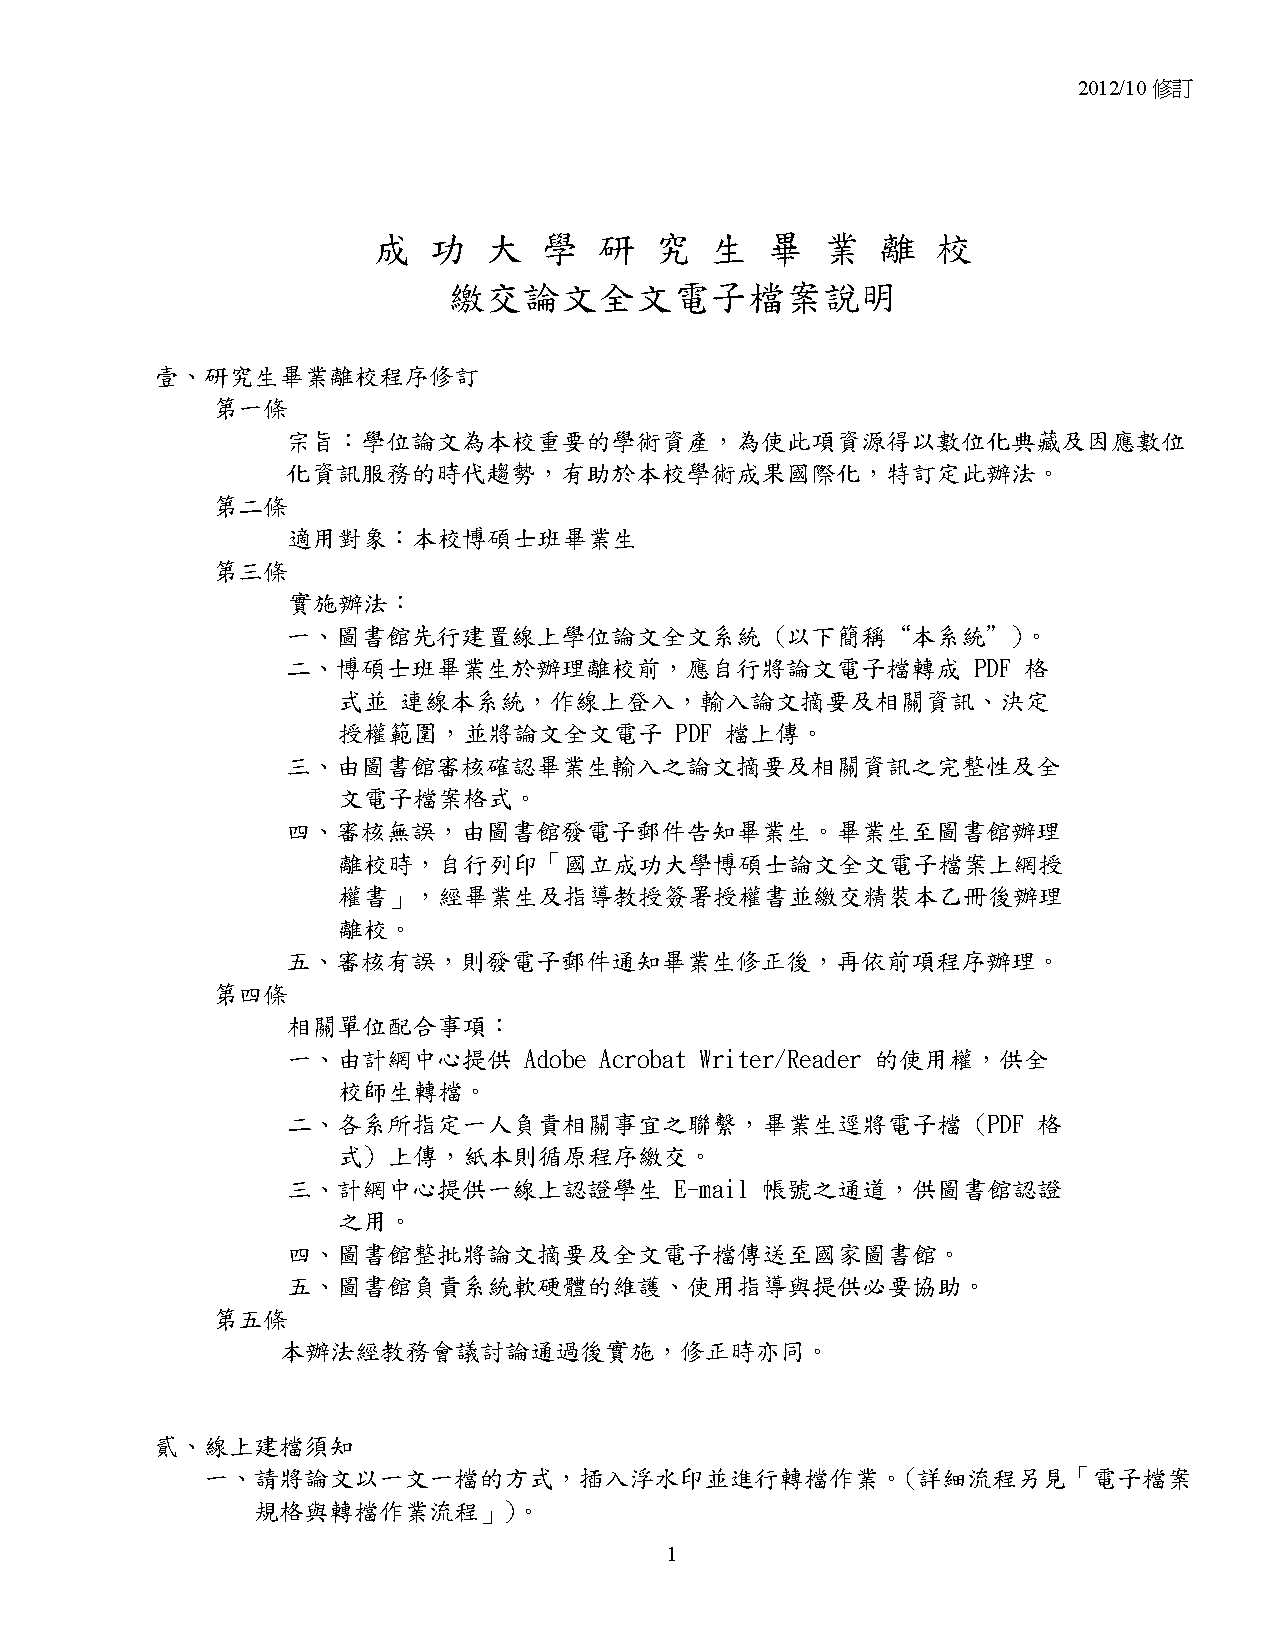
\includepdf[pages=-]{./example/appendix/pdf/2012050004-a.pdf}
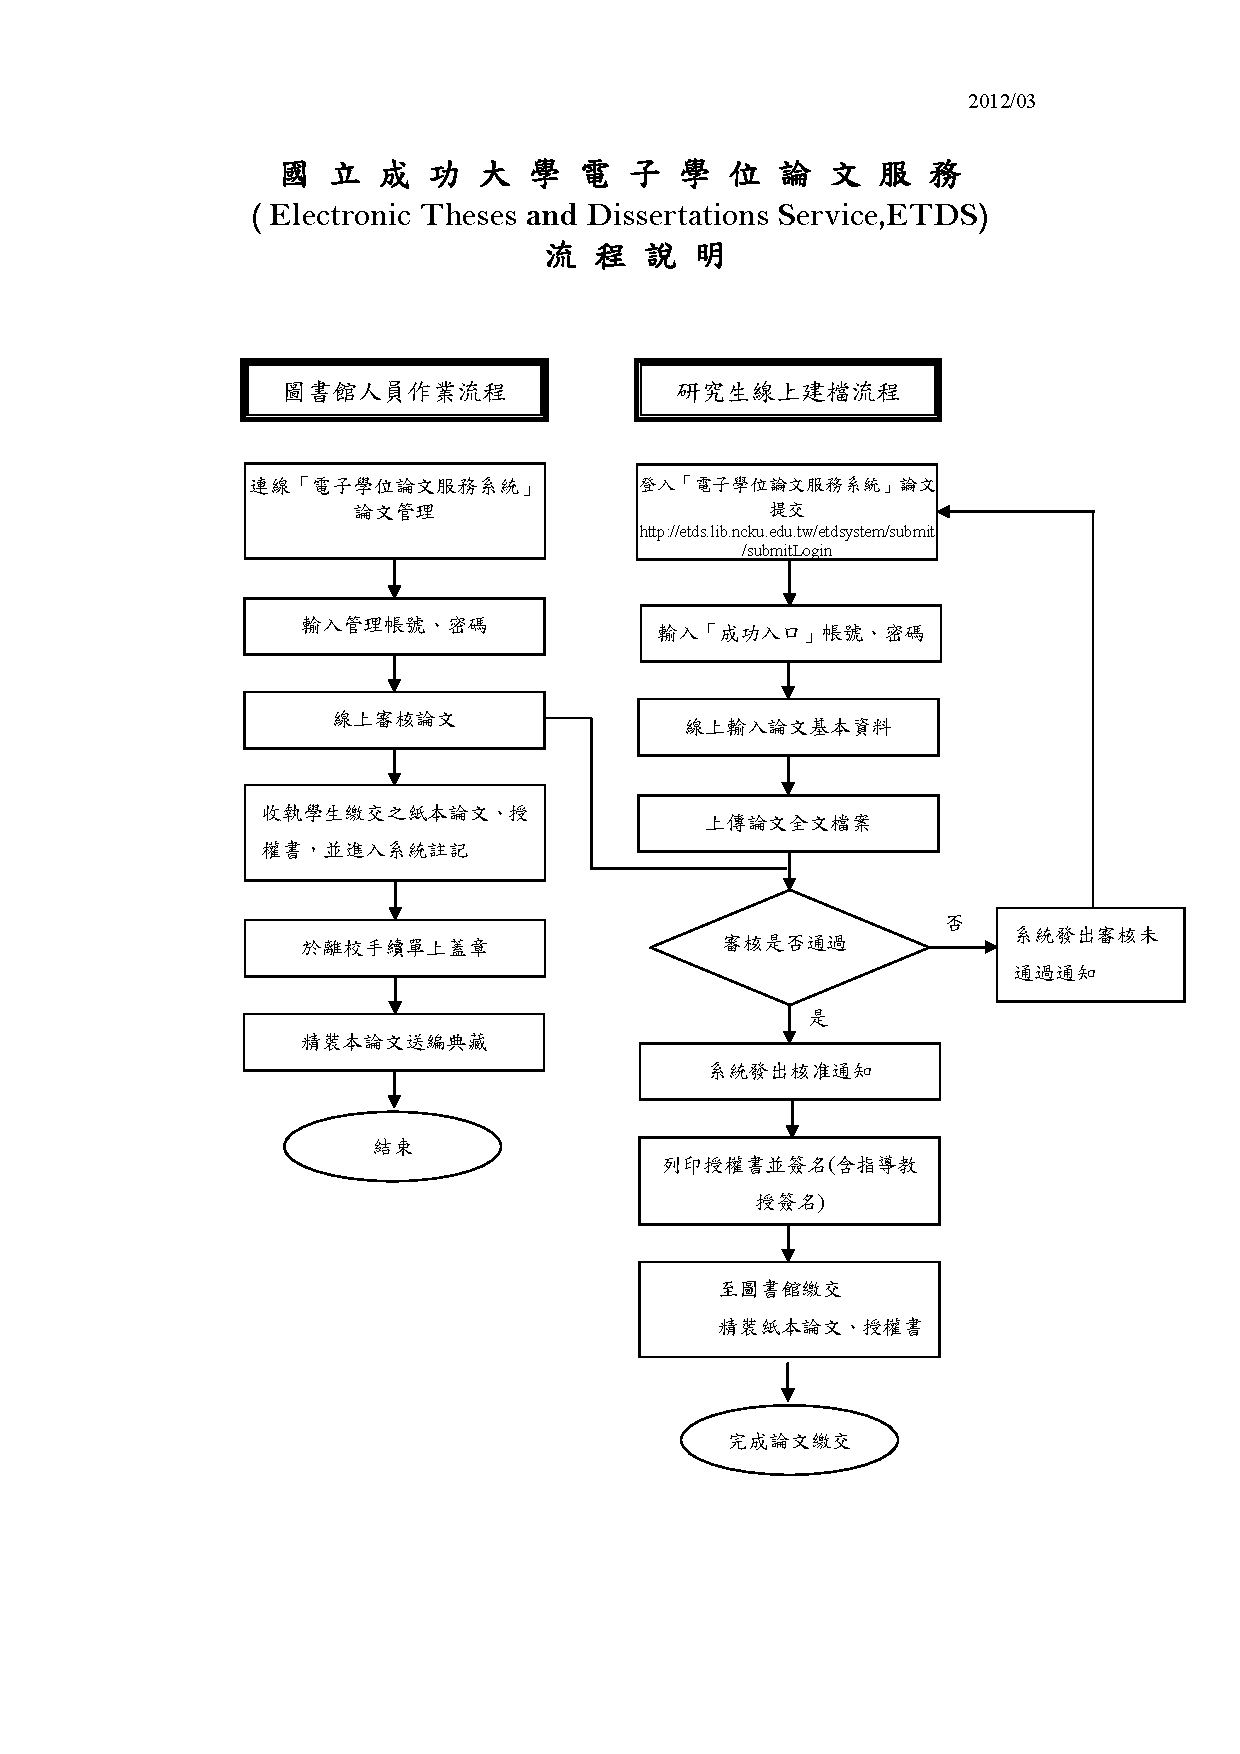
\includepdf[pages=-]{./example/appendix/pdf/2012050006-a.pdf}

% ------------------------------------------------
\EndChapter
% ------------------------------------------------

% ------------------------------------------------
% Page start
\newpage
\phantomsection
% ------------------------------------------------

\chapter{各系所博碩士撰寫論文須知}
\label{appendix:thesis-spec}

\section{介紹}
這部份資料來源是使用'電機工程系辦網頁'中的'論文撰寫須知.pdf'(\url{http://office.ee.ncku.edu.tw/uploads/%E8%AB%96%E6%96%87%E6%92%B0%E5%AF%AB%E9%A0%88%E7%9F%A5.pdf}).\\

但由於原檔案沒法顯示, 故需要另重新儲存成一個新的出來. 使用學校的Adobe Acrobat XI試驗, 發現要使用'儲存為其他->可存檔PDF (PDF/A)'才能顯示出來.\\

\begin{figure}[h]
\centering
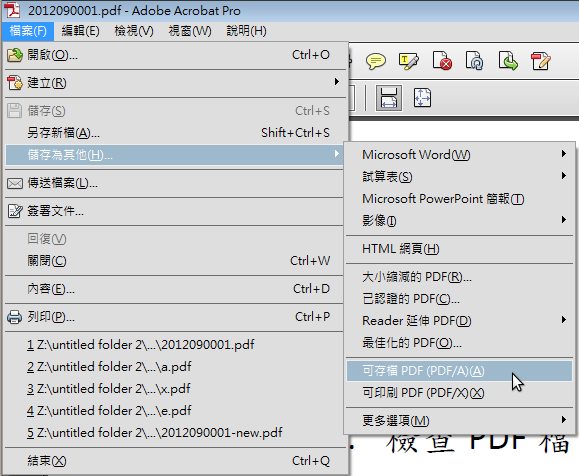
\includegraphics[scale=0.3]{./example/appendix/pic/save_pdf.png}
\caption{在Adobe Acrobat另存新版本}
\label{fig:appendix:save_pdf}
\end{figure}

檔案位置:\\
新: 'example/appendix/pdf/thesis-spec.pdf'\\
原: 'example/appendix/pdf/論文撰寫須知.pdf'\\

\setboolean{@twoside}{false}
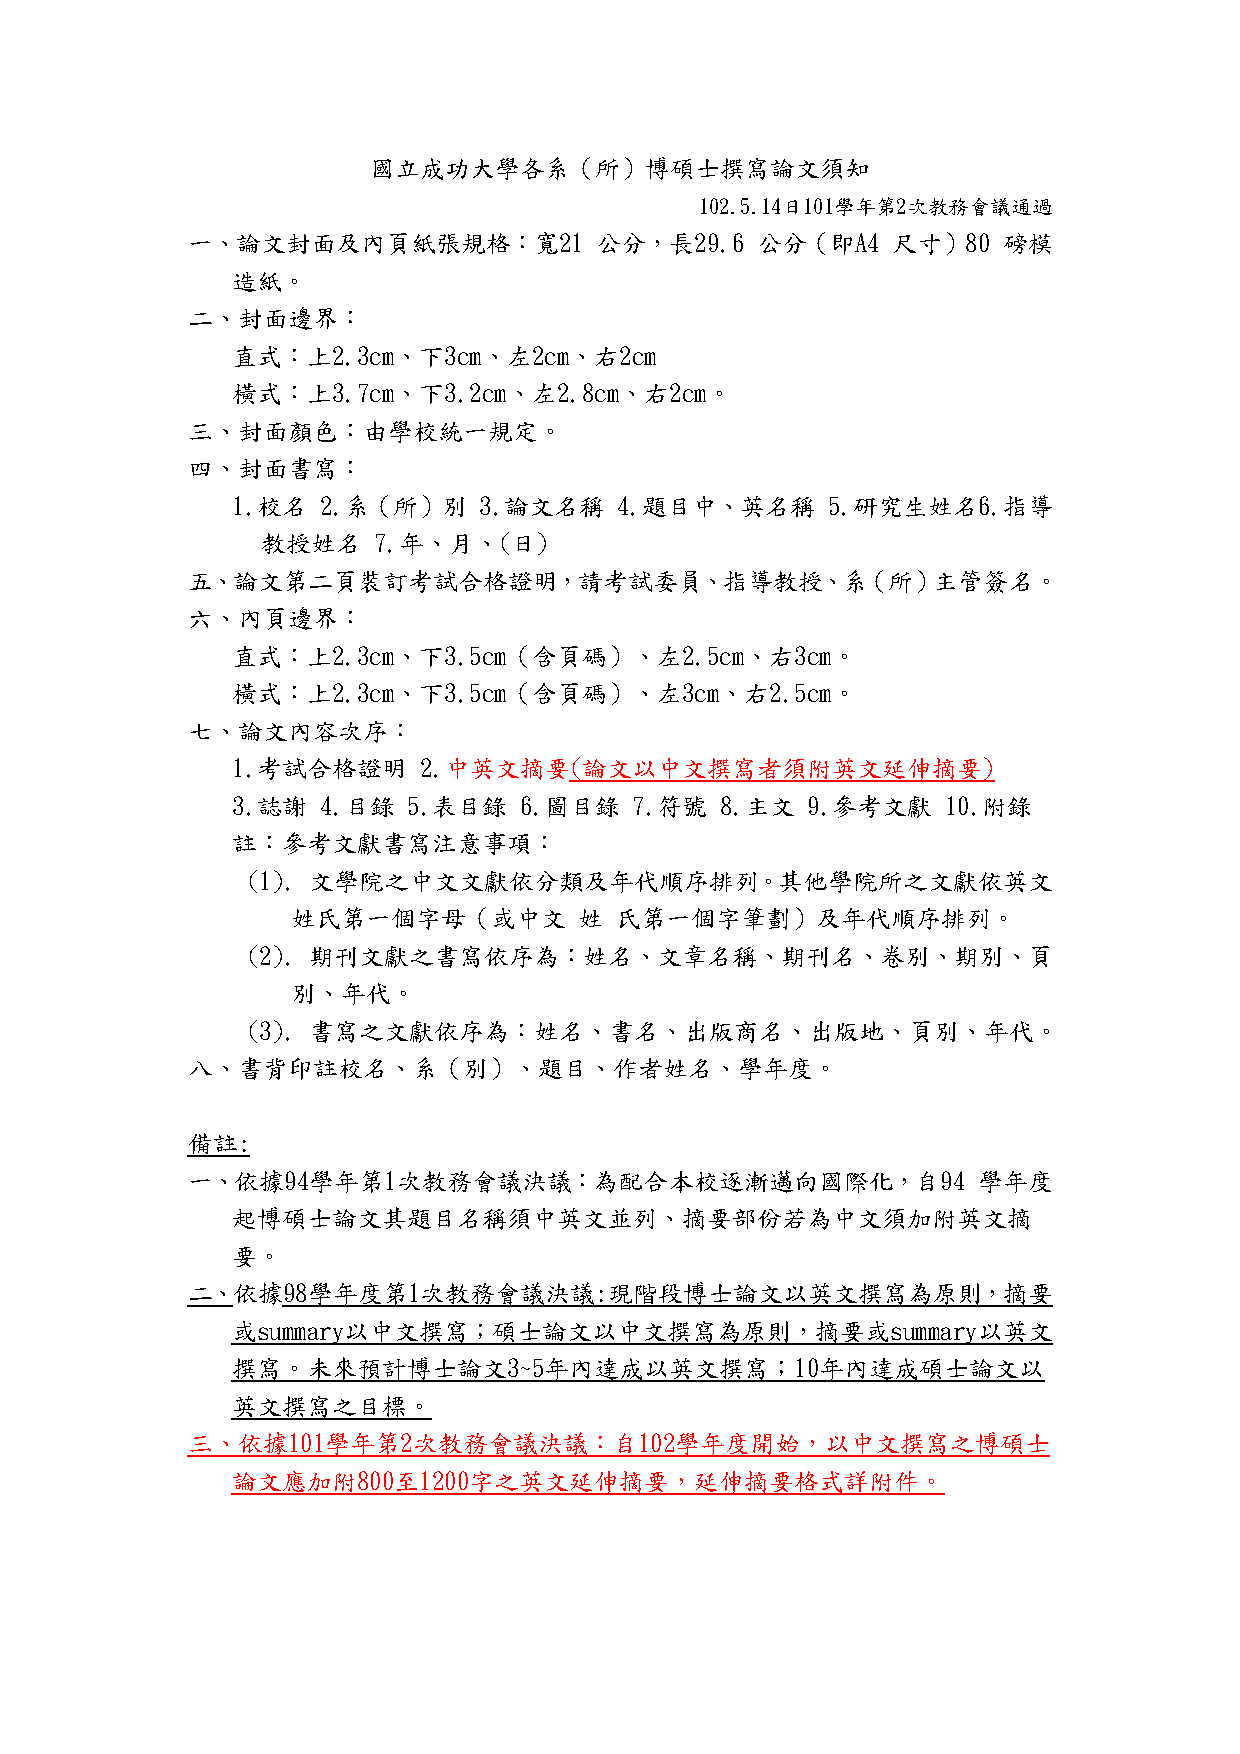
\includepdf[pages=-]{./example/appendix/pdf/thesis-spec.pdf}

% ------------------------------------------------
% End of page
% ------------------------------------------------

%% ------------------------------------------------
\StartChapter{電子論文上傳前檢查事項}{appendix:e-paper_upload}
% ------------------------------------------------

\section{介紹}
這部份資料來源是使用'成功大學電子學位論文服務'中的'電子論文上傳前檢查事項'的'2012090001.pdf'.\\

同樣原檔案沒法顯示, 故需要進行另儲存.\\

檔案位置:\\
新: 'example/appendix/pdf/2012090001-a.pdf'\\
原: 'example/appendix/pdf/2012090001.pdf'\\

\setboolean{@twoside}{false}
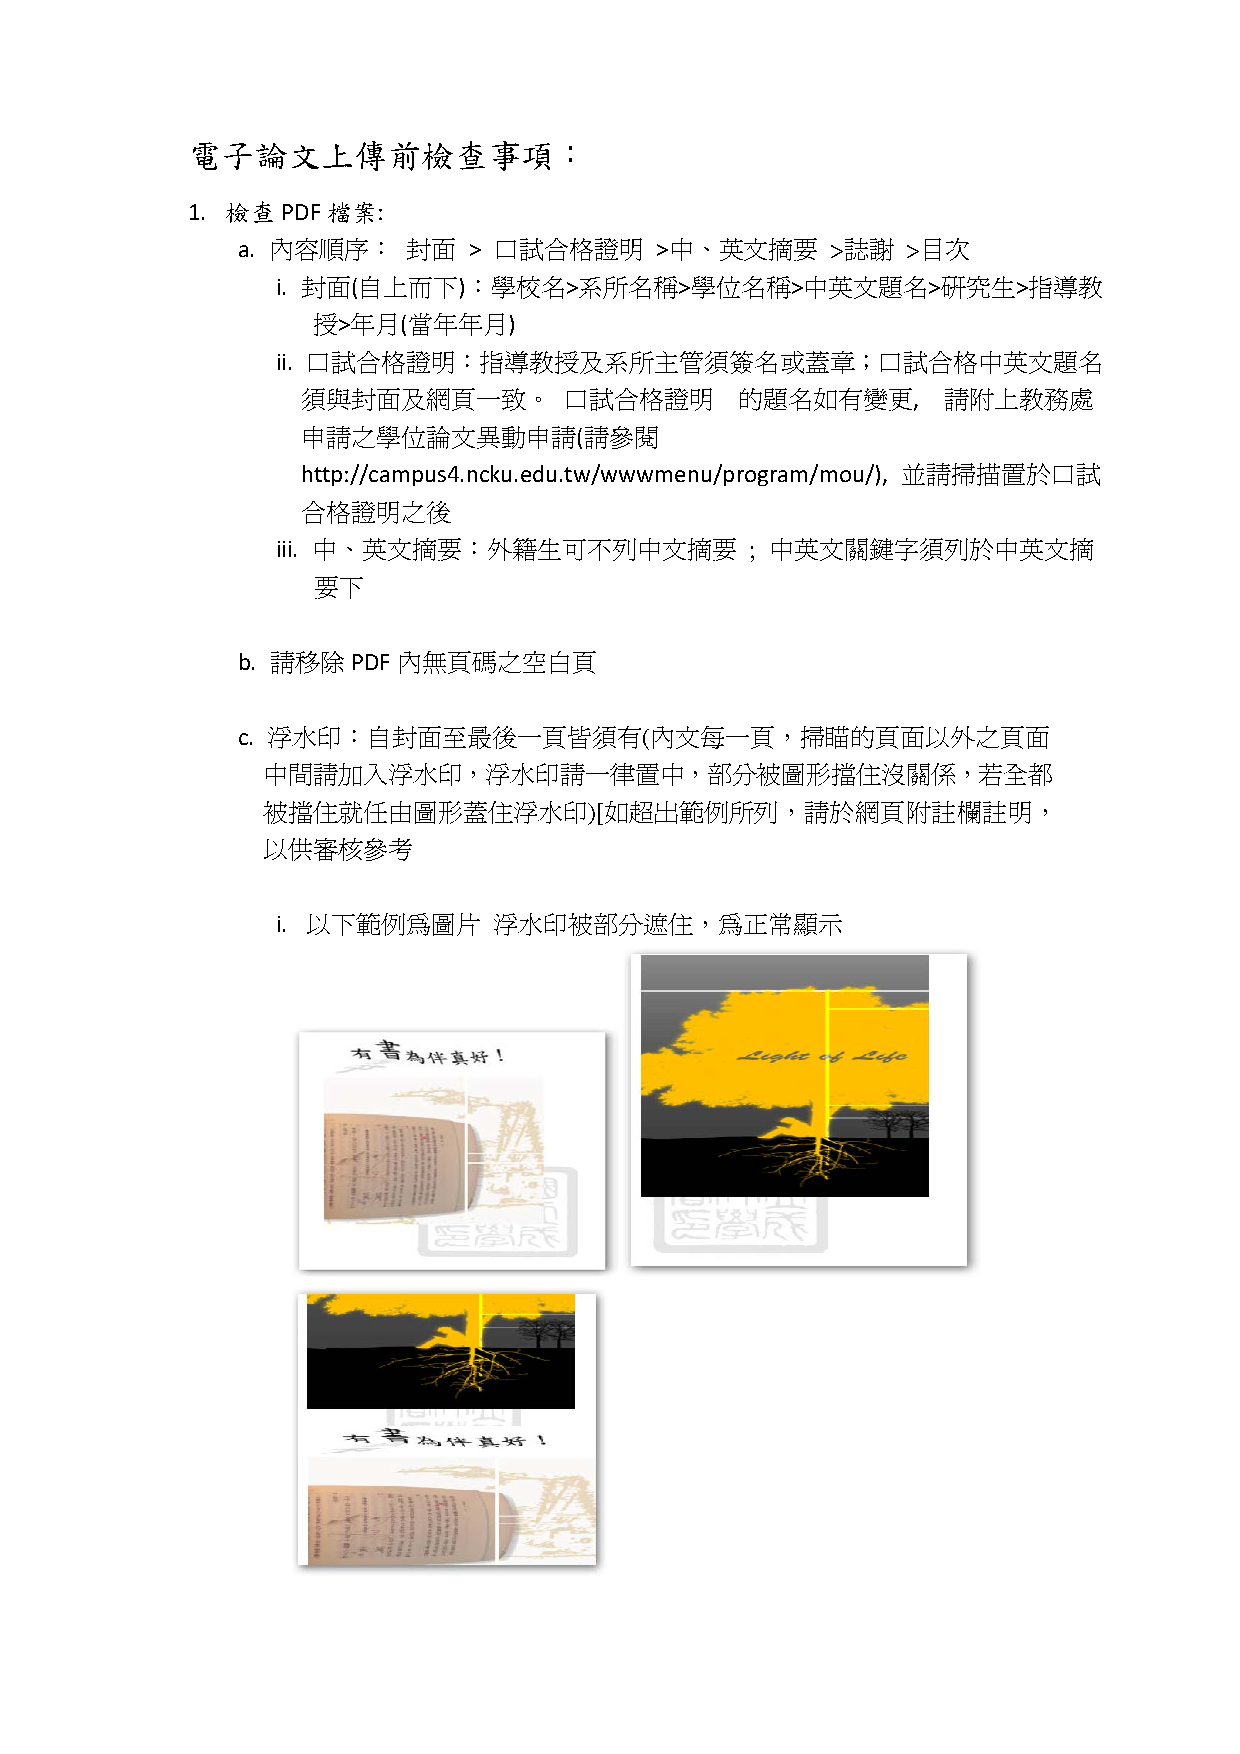
\includepdf[pages=-]{./example/appendix/pdf/2012090001-a.pdf}

% ------------------------------------------------
\EndChapter
% ------------------------------------------------

%% ------------------------------------------------
\StartChapter{學位論文上傳說明}{appendix:e-paper_upload_ppt}
% ------------------------------------------------

這部份資料來源是使用'電子學位論文服務'提供的 '2015論文提交說明簡報檔'\RefBib{web:lib:2015-submit-ppt} 修改而成的, 只抽出使用本模版後, 還要做什麼的行為.\\

\setboolean{@twoside}{false}
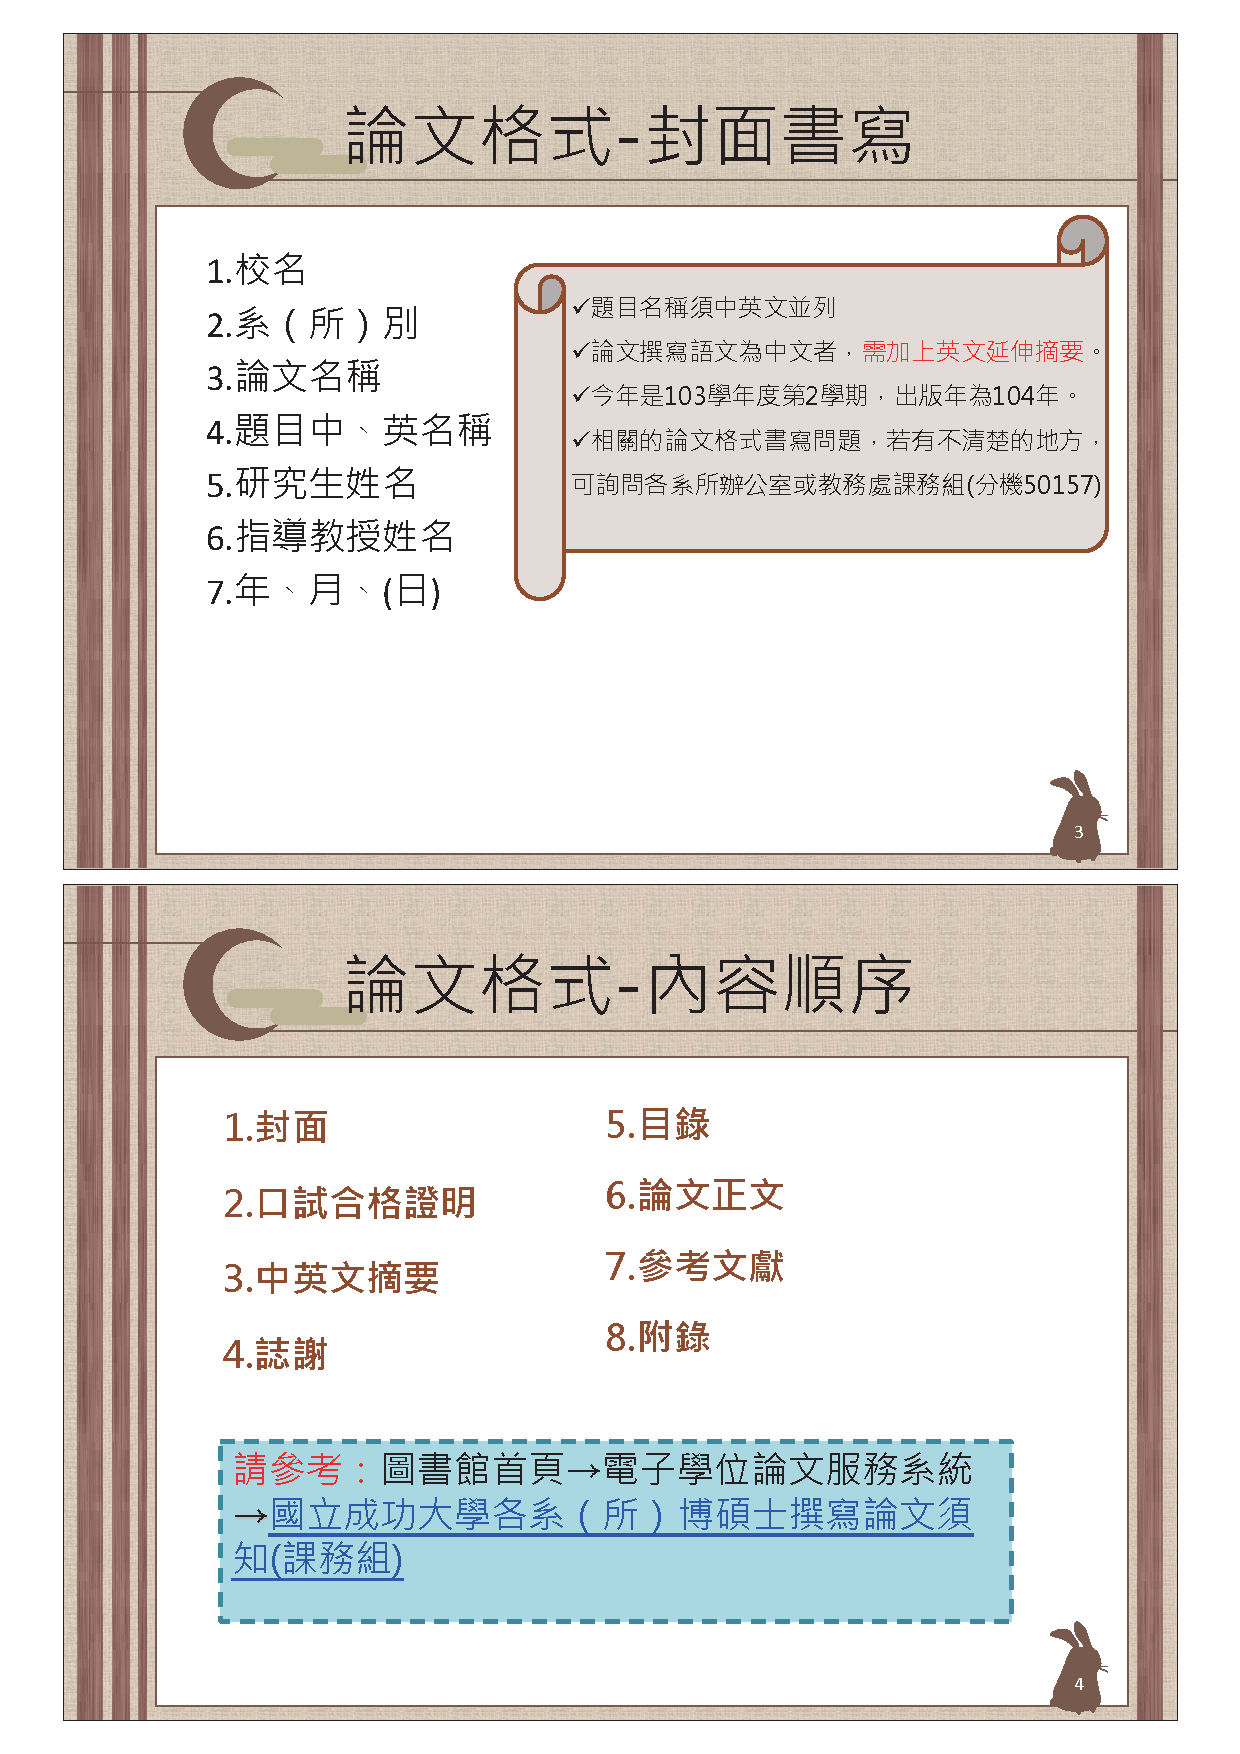
\includepdf[pages=-]{./example/appendix/pdf/2012050003-short-a}

% ------------------------------------------------
\EndChapter
% ------------------------------------------------


%% ------------------------------------------------
\StartChapter{口試注意事項}
% ------------------------------------------------

這部份資料來源是使用本系資訊工程研究所系辦所提供的資料, 雖然內容主要針對本系, 但某些內容都是適合非本系的同學們.

\setboolean{@twoside}{false}
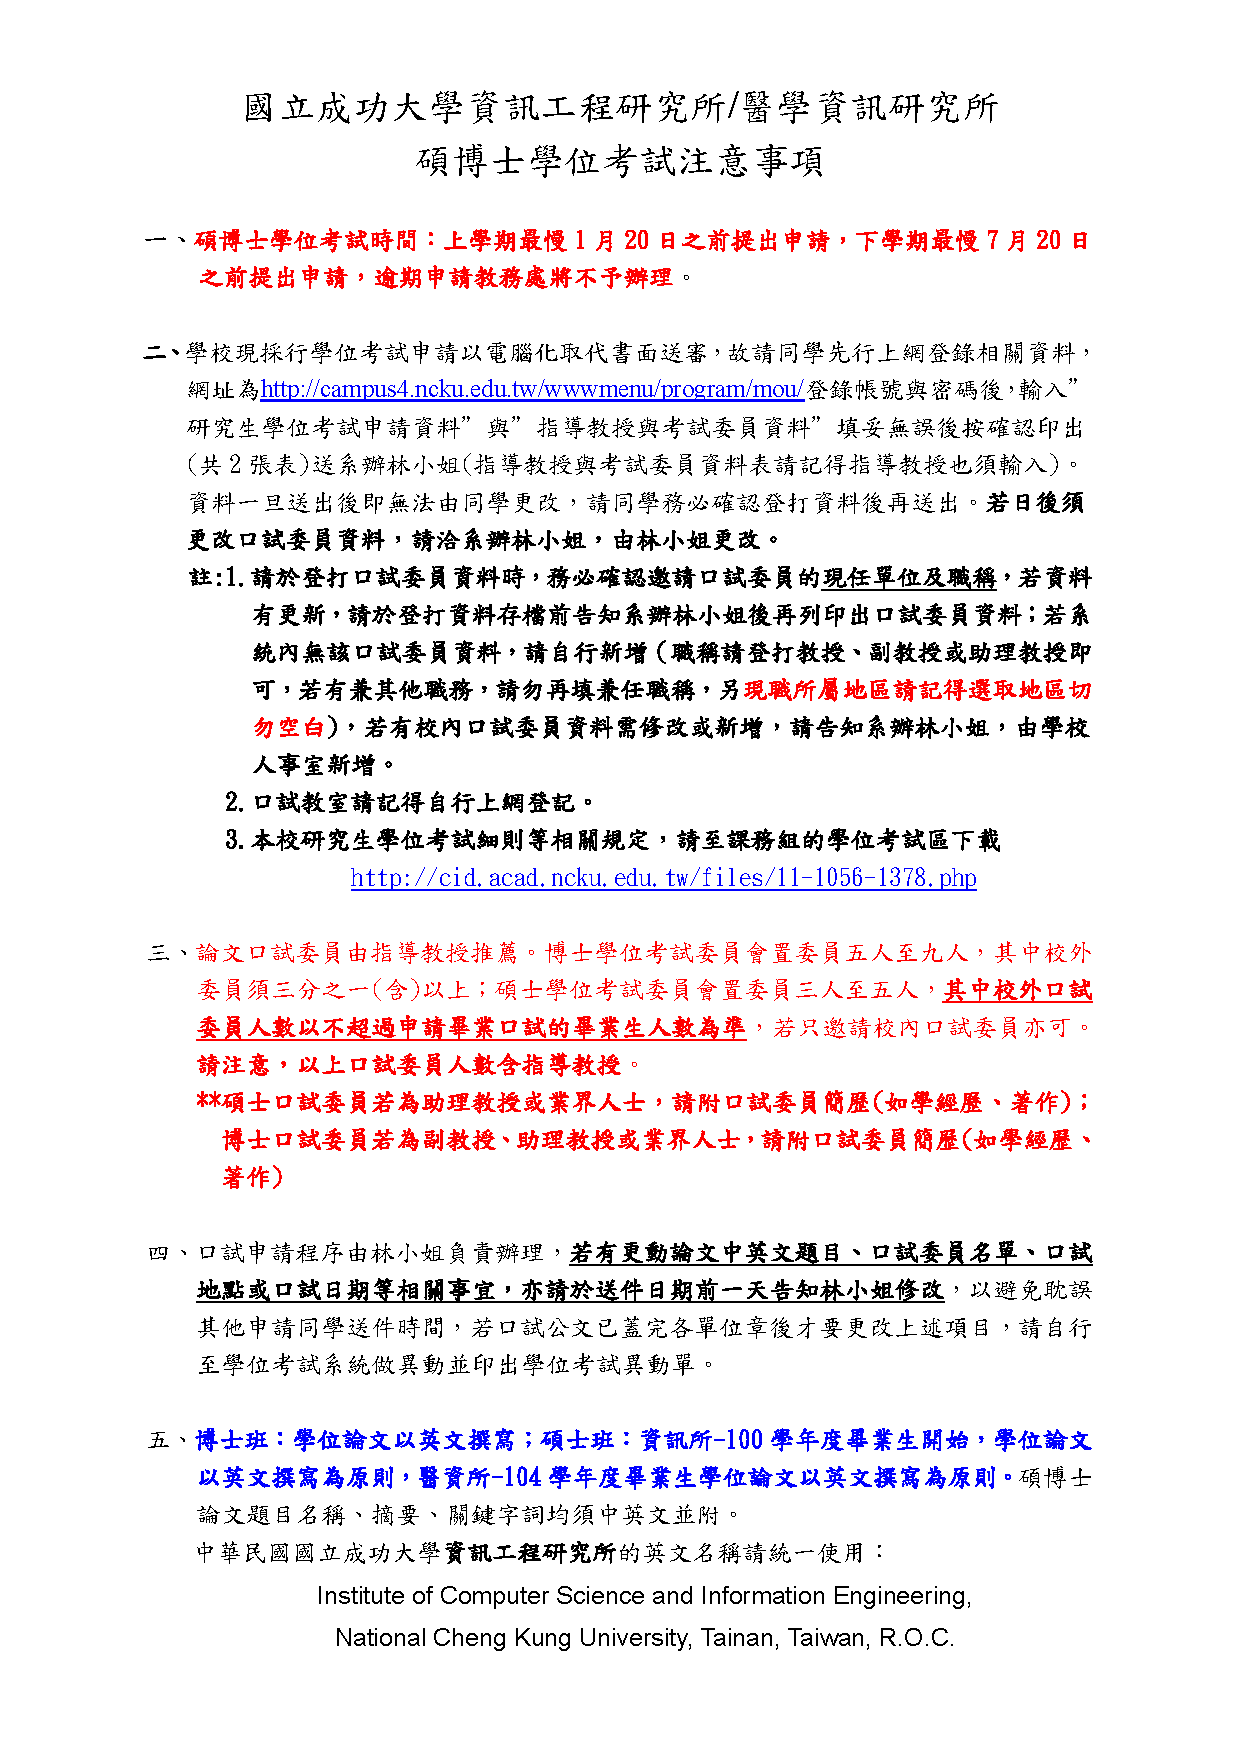
\includepdf[pages=-]{./example/appendix/pdf/oral-1040616-a.pdf}

% ------------------------------------------------
\EndChapter
% ------------------------------------------------

%% ------------------------------------------------
\StartChapter{常見問題Q\&A}{appendix:faq}
% ------------------------------------------------

\StartSection{介紹}
這部份資料來源是使用'電子學位論文服務'提供的'FAQ'\RefBib{web:lib:ETDS-QA}, 用來補充其他Appendix沒提到的一些情報.\\

\setboolean{@twoside}{false}
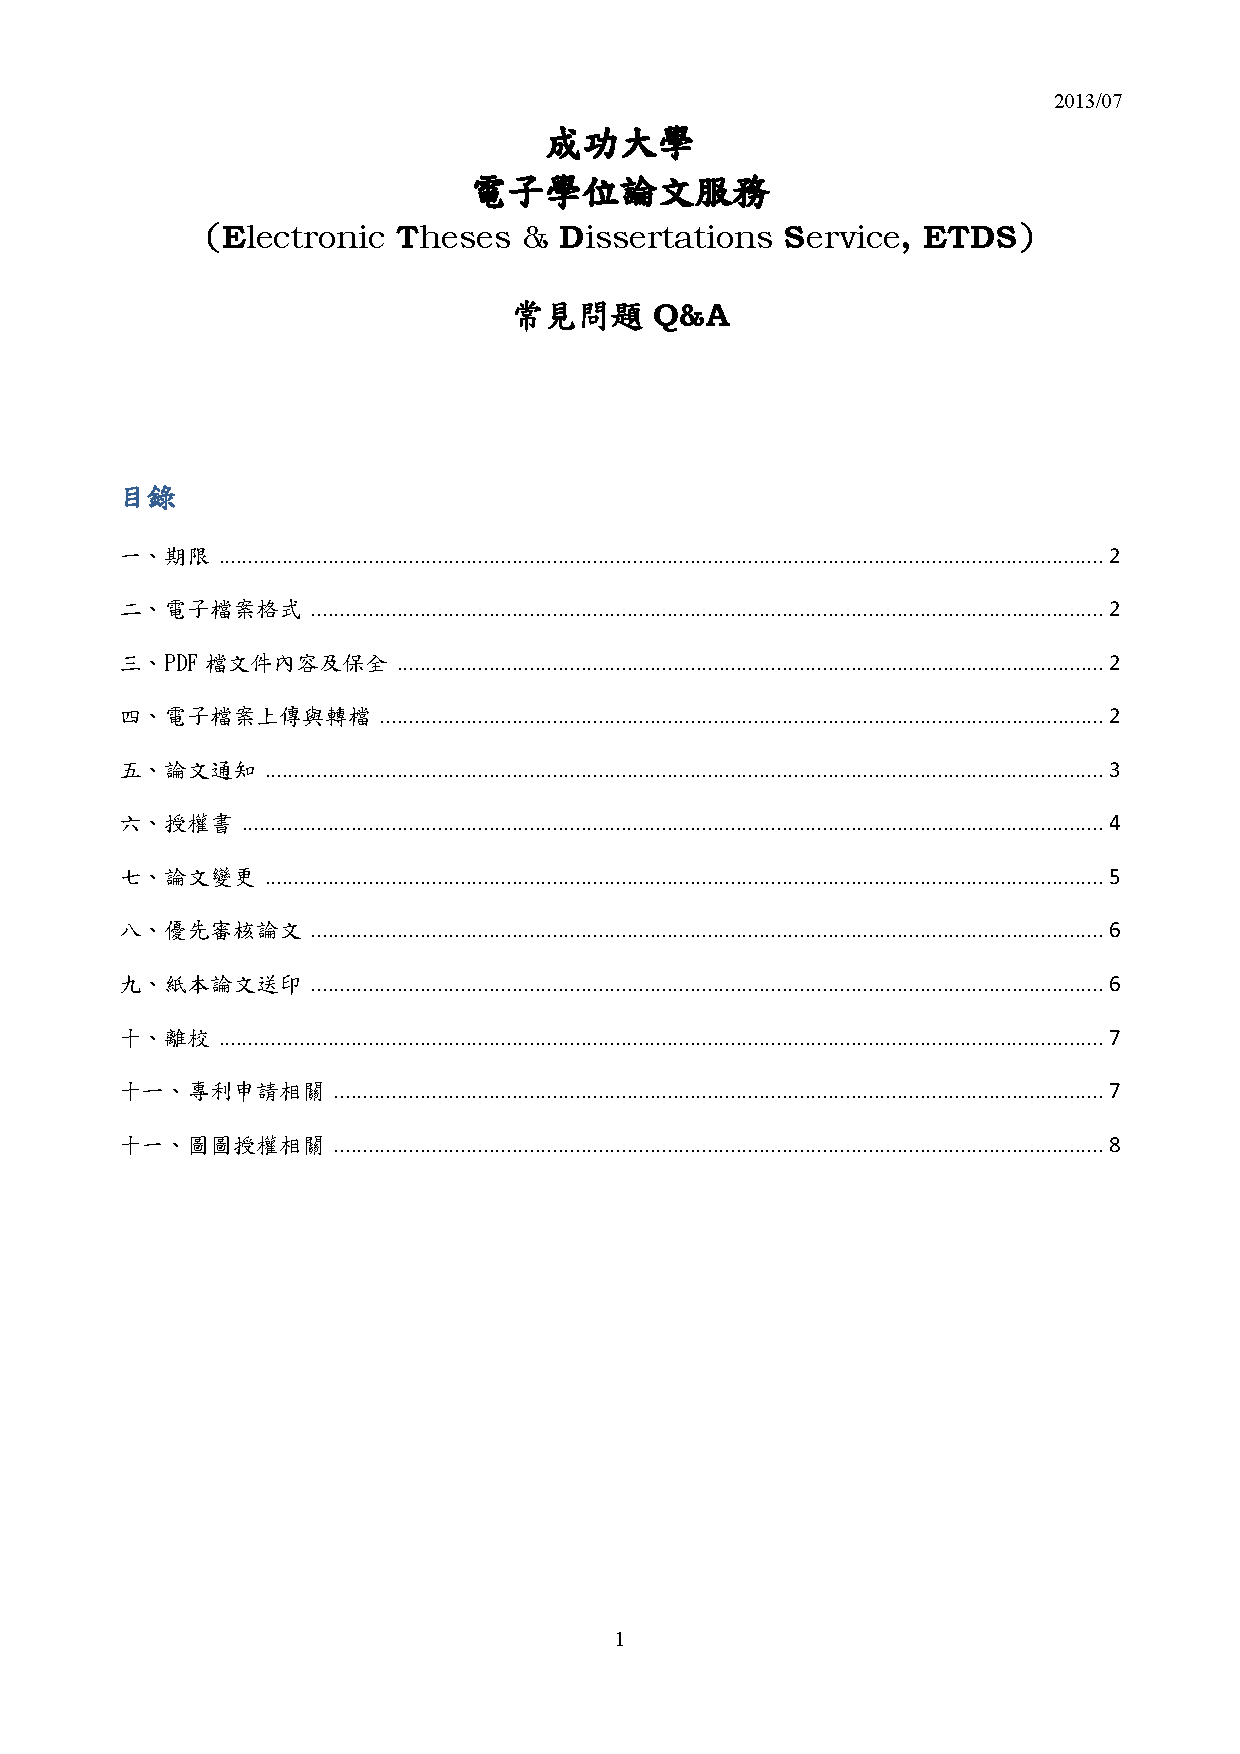
\includepdf[pages=-]{./example/appendix/pdf/2012050009-a.pdf}

% ------------------------------------------------
\EndChapter
% ------------------------------------------------

%% ------------------------------------------------
\StartChapter{LaTex Symbol寫法}{appendix:unicode-symbols}
% ------------------------------------------------

這部份資料來源是xeCJK的v3.3.4(2016/02/10)版本中提供的50頁有關所有Symbol的寫法, 極度值得同學們閱讀或在這邊找你所需的Symbols.\\

內容的說明方式為:\\
Symbol: 符號所顯示的樣子\\
USV: 以Unicode方式所代表的這個符號, 例如 `(' 的Unicode寫法為U+0028.\\
Description: 是這符號的名字.\\
Macro(s): 是LaTex使用這符號的寫法.\\

\textbf{P.S: }因為符號數量多, 沒法100\%保證全能使用.

\setboolean{@twoside}{false}
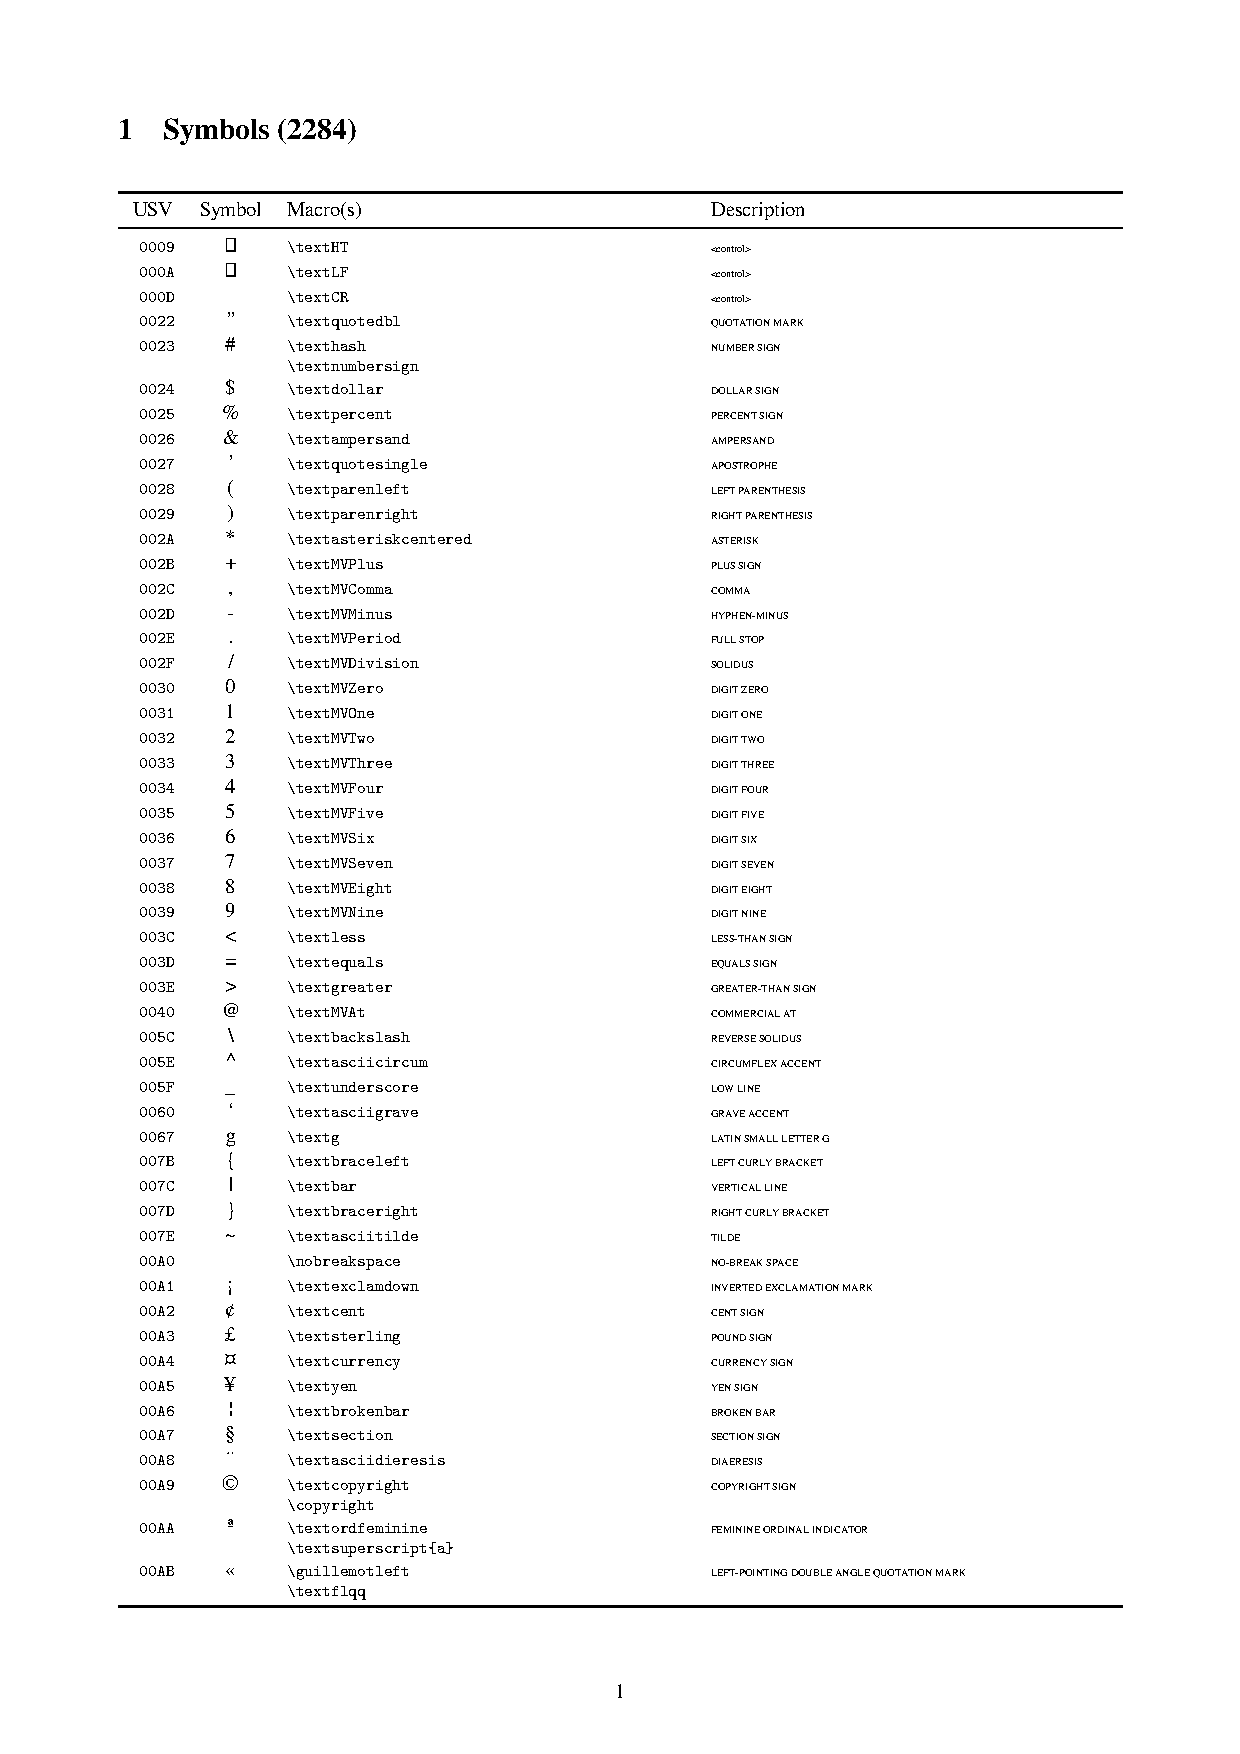
\includepdf[pages=-]{./example/appendix/pdf/xunicode-symbols.pdf}

% ------------------------------------------------
\EndChapter
% ------------------------------------------------


% ------------------------------------------------
\EndAppendix
% ------------------------------------------------


% ------------------------------------------------

% 用來對內容進行不同的設定測試用的測試頁
%
% Reference from:
%
% 半形字元與全形字元
% <https://zh.wikipedia.org/wiki/%E5%85%A8%E5%BD%A2%E5%92%8C%E5%8D%8A%E5%BD%A2>
%
% ------------------------------------------------
\StartChapter{測試頁 Testing Pages}
% ------------------------------------------------

這邊是用來放置不同的內容來進行測試或設計樣版用的.

% ------------------------------------------------

\StartSection{半形字元與全形字元的比較 (ASCII字元)}
用來檢查半形/全形字元顯示正常\\

\begin{verbatim}
   全形    半形        |        全形    半形        |        全形    半形
   " "     " "                 !       !                  "       "
    #       #                  $       $                  %       %
    &       &                  '       '                  (       (
    )       )                  *       *                  +       +
    ,       ,                  -       -                  .       .
    /       /

    0       0                 1       1                  2       2
    3       3                 4       4                  5       5
    6       6                 7       7                  8       8
    9       9

    :       :                 ;       ;                  <       <
    =       =                 >       >                  ?       ?
    @       @

    A       A                 B       B                  C       C
    D       D                 E       E                  F       F
    G       G                 H       H                  I       I
    J       J                 K       K                  L       L
    M       M                 N       N                  O       O
    P       P                 Q       Q                  R       R
    S       S                 T       T                  U       U
    V       V                 W       W                  X       X
    Y       Y                 Z       Z

    [       [                 \       \                  ]       ]
    ^       ^                 _       _                  `       `

    a       a                 b       b                  c       c
    d       d                 e       e                  f       f
    g       g                 h       h                  i       i
    j       j                 k       k                  l       l
    m       m                 n       n                  o       o
    p       p                 q       q                  r       r
    s       s                 t       t                  u       u
    v       v                 w       w                  x       x
    y       y                 z       z

    {       {                 |       |                  }       }
    ~       ~
\end{verbatim}

% ------------------------------------------------

\UseEngLinesSpacing

\newpage
\StartSection{英文內容 (只用段落來分段)}
用來看內容, 符號, 段距, 字元之間的距離等東西\\

NCKU offers an open learning environment characterized by classical Western and modern eastern landscape. NCKU has attracted numerous distinguished visitors around the world for its rich and welcoming campuses.

In addition to two off-university campuses, An-Nan and Gueiren, the main campus of NCKU consists of 7 satellite campuses adjacent to one another. NCKU occupies a total of more than 180 hectares of land, which tops many other universities in Taiwan. NCKU started out as having only one campus, Cheng Kung, but continued to expand to its current scale. Each campus in the major part of NCKU is closely interlinked and tightly developed as a city within the university.

NCKU's spirit of ``pristine practicality'' and its motto of ``intellectual development through persistent pursuit of knowledge'' have been intrinsic to the thick cultural heritage of the city of Tainan. While members of NCKU are well-integrated with one another, they also work independently. Patrons as NCKU enjoy abundant learning resources.

Through continuous evolution and progression, NCKU has become an active participant in global academia and has earned an excellent reputation in teaching and research. For example, NCKU has ranked the 256th in 2010 Academic Ranking of World Universities announced by Shanghai Jiaotong University and the 80th in 2011 Webometrics Ranking of World Universities published by Centre for Scientific Information and Documentation, Spain, only second to that of NTU, Todai and Kyodai in the Asian region.


% ------------------------------------------------

\newpage
\StartSection{英文內容 (只用強制斷行)}
用來看內容, 符號, 段距, 字元之間的距離等東西\\

NCKU offers an open learning environment characterized by classical Western and modern eastern landscape. NCKU has attracted numerous distinguished visitors around the world for its rich and welcoming campuses.\\
In addition to two off-university campuses, An-Nan and Gueiren, the main campus of NCKU consists of 7 satellite campuses adjacent to one another. NCKU occupies a total of more than 180 hectares of land, which tops many other universities in Taiwan. NCKU started out as having only one campus, Cheng Kung, but continued to expand to its current scale. Each campus in the major part of NCKU is closely interlinked and tightly developed as a city within the university.\\
NCKU's spirit of ``pristine practicality'' and its motto of ``intellectual development through persistent pursuit of knowledge'' have been intrinsic to the thick cultural heritage of the city of Tainan. While members of NCKU are well-integrated with one another, they also work independently. Patrons as NCKU enjoy abundant learning resources.\\
Through continuous evolution and progression, NCKU has become an active participant in global academia and has earned an excellent reputation in teaching and research. For example, NCKU has ranked the 256th in 2010 Academic Ranking of World Universities announced by Shanghai Jiaotong University and the 80th in 2011 Webometrics Ranking of World Universities published by Centre for Scientific Information and Documentation, Spain, only second to that of NTU, Todai and Kyodai in the Asian region.


% ------------------------------------------------

\newpage
\StartSection{英文內容 (段落 + 強制斷行)}
用來看內容, 符號, 段距, 字元之間的距離等東西\\

NCKU offers an open learning environment characterized by classical Western and modern eastern landscape. NCKU has attracted numerous distinguished visitors around the world for its rich and welcoming campuses.\\

In addition to two off-university campuses, An-Nan and Gueiren, the main campus of NCKU consists of 7 satellite campuses adjacent to one another. NCKU occupies a total of more than 180 hectares of land, which tops many other universities in Taiwan. NCKU started out as having only one campus, Cheng Kung, but continued to expand to its current scale. Each campus in the major part of NCKU is closely interlinked and tightly developed as a city within the university.\\

NCKU's spirit of ``pristine practicality'' and its motto of ``intellectual development through persistent pursuit of knowledge'' have been intrinsic to the thick cultural heritage of the city of Tainan. While members of NCKU are well-integrated with one another, they also work independently. Patrons as NCKU enjoy abundant learning resources.\\

Through continuous evolution and progression, NCKU has become an active participant in global academia and has earned an excellent reputation in teaching and research. For example, NCKU has ranked the 256th in 2010 Academic Ranking of World Universities announced by Shanghai Jiaotong University and the 80th in 2011 Webometrics Ranking of World Universities published by Centre for Scientific Information and Documentation, Spain, only second to that of NTU, Todai and Kyodai in the Asian region.

% ------------------------------------------------

\UseChiLinesSpacing

\newpage
\StartSection{中文內容 (只用段落來分段)}
用來看內容, 符號, 段距, 字元之間的距離等東西\\

本校創校於西元1931年(昭和6年,民國20年)1月15日,原名為「臺南高等工業學校」;1944年(昭和19年,民國33年)改稱為「臺南工業專門學校」。民國34年臺灣光復。本校於民國35年2月改制為「臺灣省立臺南工業專科學校」,由王石安博士擔任校長;35年10月改制為「臺灣省立工學院」,仍由王石安博士擔任校長。彼時僅有成功校區,39年增購勝利校區。41年2月,由秦大鈞博士接任校長。

45年8月,本校改制為「臺灣省立成功大學」,仍由秦大鈞博士擔任校長;同時增設文理學院及商學院。46年8月,由閻振興博士接任校長。54年1月,由羅雲平博士接任校長。55年增購光復校區。58年10月,將文理學院分為文學院及理學院。60年8月,改制為「國立成功大學」,並由倪超博士接任校長;同年增購建國校區。67年8月,由王唯農博士接任校長。

69年8月,夏漢民博士接任校長;同年將商學院更名為管理學院。72年8月,增設醫學院,並增購自強校區及敬業校區。74年增購力行校區部分校地。76年增購歸仁校區,設置航空太空實驗場。77年6月本校醫學院附設醫院正式營運。77年8月,馬哲儒博士接任校長。80年增購自強校區北半部。82年陸續增購台南市「文大五」用地,闢為本校安南校區。

83年8月,吳京院士接任校長。吳校長於85年6月入閣擔任教育部長,由副校長黃定加博士代理校長。86年2月,翁政義博士接任校長。86年8月增設社會科學院。88年完成收購安南校區全部校地;同年6月增購原陸軍八○四醫院用地(91年6月完成撥用手續)。翁校長於89年5月出任國科會主委,由副校長翁鴻山博士代理校長。90年2月,高強博士接任校長。92年8月,增設電機資訊學院、規劃與設計學院。94年7月,本校配合國軍斗六醫院精實案,接管該院營運權,設置為雲林縣斗六校區,並改制為本校醫學院附設醫院斗六分院。94年8月,增設生物科學與科技學院。94年10月,本校得到教育部的肯定,獲選為「發展國際一流大學及頂尖研究中心計畫」的兩所重點大學之一。

96年2月,賴明詔院士接任校長,97年2月教育部公佈「發展國際一流大學及頂尖研究中心計畫」第二梯次的審議結果,本校繼續獲得教育部的肯定與補助,積極朝國際一流大學的目標邁進。97年10月增購歸仁校區北側台糖土地(正式登記為本校管有)。100年2月,黃煌煇博士接任校長。100年4月本校獲得教育部第二期頂尖大學計畫補助,持續朝國際一流大學的目標邁進。104年2月,蘇慧貞博士接任校長。

% ------------------------------------------------

\newpage
\StartSection{中文內容 (只用強制斷行)}
用來看內容, 符號, 段距, 字元之間的距離等東西\\

本校創校於西元1931年(昭和6年,民國20年)1月15日,原名為「臺南高等工業學校」;1944年(昭和19年,民國33年)改稱為「臺南工業專門學校」。民國34年臺灣光復。本校於民國35年2月改制為「臺灣省立臺南工業專科學校」,由王石安博士擔任校長;35年10月改制為「臺灣省立工學院」,仍由王石安博士擔任校長。彼時僅有成功校區,39年增購勝利校區。41年2月,由秦大鈞博士接任校長。\\
45年8月,本校改制為「臺灣省立成功大學」,仍由秦大鈞博士擔任校長;同時增設文理學院及商學院。46年8月,由閻振興博士接任校長。54年1月,由羅雲平博士接任校長。55年增購光復校區。58年10月,將文理學院分為文學院及理學院。60年8月,改制為「國立成功大學」,並由倪超博士接任校長;同年增購建國校區。67年8月,由王唯農博士接任校長。\\
69年8月,夏漢民博士接任校長;同年將商學院更名為管理學院。72年8月,增設醫學院,並增購自強校區及敬業校區。74年增購力行校區部分校地。76年增購歸仁校區,設置航空太空實驗場。77年6月本校醫學院附設醫院正式營運。77年8月,馬哲儒博士接任校長。80年增購自強校區北半部。82年陸續增購台南市「文大五」用地,闢為本校安南校區。\\
83年8月,吳京院士接任校長。吳校長於85年6月入閣擔任教育部長,由副校長黃定加博士代理校長。86年2月,翁政義博士接任校長。86年8月增設社會科學院。88年完成收購安南校區全部校地;同年6月增購原陸軍八○四醫院用地(91年6月完成撥用手續)。翁校長於89年5月出任國科會主委,由副校長翁鴻山博士代理校長。90年2月,高強博士接任校長。92年8月,增設電機資訊學院、規劃與設計學院。94年7月,本校配合國軍斗六醫院精實案,接管該院營運權,設置為雲林縣斗六校區,並改制為本校醫學院附設醫院斗六分院。94年8月,增設生物科學與科技學院。94年10月,本校得到教育部的肯定,獲選為「發展國際一流大學及頂尖研究中心計畫」的兩所重點大學之一。\\
96年2月,賴明詔院士接任校長,97年2月教育部公佈「發展國際一流大學及頂尖研究中心計畫」第二梯次的審議結果,本校繼續獲得教育部的肯定與補助,積極朝國際一流大學的目標邁進。97年10月增購歸仁校區北側台糖土地(正式登記為本校管有)。100年2月,黃煌煇博士接任校長。100年4月本校獲得教育部第二期頂尖大學計畫補助,持續朝國際一流大學的目標邁進。104年2月,蘇慧貞博士接任校長。

% ------------------------------------------------

\newpage
\StartSection{中文內容 (段落 + 強制斷行)}
用來看內容, 符號, 段距, 字元之間的距離等東西\\

本校創校於西元1931年(昭和6年,民國20年)1月15日,原名為「臺南高等工業學校」;1944年(昭和19年,民國33年)改稱為「臺南工業專門學校」。民國34年臺灣光復。本校於民國35年2月改制為「臺灣省立臺南工業專科學校」,由王石安博士擔任校長;35年10月改制為「臺灣省立工學院」,仍由王石安博士擔任校長。彼時僅有成功校區,39年增購勝利校區。41年2月,由秦大鈞博士接任校長。\\

45年8月,本校改制為「臺灣省立成功大學」,仍由秦大鈞博士擔任校長;同時增設文理學院及商學院。46年8月,由閻振興博士接任校長。54年1月,由羅雲平博士接任校長。55年增購光復校區。58年10月,將文理學院分為文學院及理學院。60年8月,改制為「國立成功大學」,並由倪超博士接任校長;同年增購建國校區。67年8月,由王唯農博士接任校長。\\

69年8月,夏漢民博士接任校長;同年將商學院更名為管理學院。72年8月,增設醫學院,並增購自強校區及敬業校區。74年增購力行校區部分校地。76年增購歸仁校區,設置航空太空實驗場。77年6月本校醫學院附設醫院正式營運。77年8月,馬哲儒博士接任校長。80年增購自強校區北半部。82年陸續增購台南市「文大五」用地,闢為本校安南校區。\\

83年8月,吳京院士接任校長。吳校長於85年6月入閣擔任教育部長,由副校長黃定加博士代理校長。86年2月,翁政義博士接任校長。86年8月增設社會科學院。88年完成收購安南校區全部校地;同年6月增購原陸軍八○四醫院用地(91年6月完成撥用手續)。翁校長於89年5月出任國科會主委,由副校長翁鴻山博士代理校長。90年2月,高強博士接任校長。92年8月,增設電機資訊學院、規劃與設計學院。94年7月,本校配合國軍斗六醫院精實案,接管該院營運權,設置為雲林縣斗六校區,並改制為本校醫學院附設醫院斗六分院。94年8月,增設生物科學與科技學院。94年10月,本校得到教育部的肯定,獲選為「發展國際一流大學及頂尖研究中心計畫」的兩所重點大學之一。\\

96年2月,賴明詔院士接任校長,97年2月教育部公佈「發展國際一流大學及頂尖研究中心計畫」第二梯次的審議結果,本校繼續獲得教育部的肯定與補助,積極朝國際一流大學的目標邁進。97年10月增購歸仁校區北側台糖土地(正式登記為本校管有)。100年2月,黃煌煇博士接任校長。100年4月本校獲得教育部第二期頂尖大學計畫補助,持續朝國際一流大學的目標邁進。104年2月,蘇慧貞博士接任校長。

% ------------------------------------------------
\UseDefaultLinesSpacing
% ------------------------------------------------

\UseChiLinesSpacing

\newpage
\StartSection{混合的中英文內容 (只用段落來分段)}
用來看內容, 符號, 段距, 字元之間的距離等東西\\

Google公司(英語:Google Inc.; 中文:穀歌[3]、穀歌[4]、科高[5]), 是一家美國的跨國科技企業, 業務範圍涵蓋互聯網搜索、雲計算、廣告技術等領域, 開發並提供大量基於互聯網的產品與服務[6], 其主要利潤來自於AdWords等廣告服務[7][8].

\begin{description}
\item [Google] Google由在斯坦福大學攻讀理工博士的拉裡•佩奇和謝爾蓋•布林共同創建, 因此兩人也被稱為``Google Guys''[9][10][11]. 1998年9月4日, Google以私營公司的形式創立, 目的是設計並管理互聯網搜尋引擎``Google搜索''. 2004年8月19日, Google公司在納斯達克上市, 後來被稱為``三駕馬車''的公司兩位共同創始人與出任首席執行官的埃裡克•施密特在此時承諾:共同在Google工作至少二十年, 即至2024年止[12].

\item [Google]\hfill\\ Google由在斯坦福大學攻讀理工博士的拉裡•佩奇和謝爾蓋•布林共同創建, 因此兩人也被稱為``Google Guys''[9][10][11]. 1998年9月4日, Google以私營公司的形式創立, 目的是設計並管理互聯網搜尋引擎``Google搜索''. 2004年8月19日, Google公司在納斯達克上市, 後來被稱為``三駕馬車''的公司兩位共同創始人與出任首席執行官的埃裡克•施密特在此時承諾:共同在Google工作至少二十年, 即至2024年止[12].

\item Google的宗旨是``整合全球範圍的資訊, 使人人皆可訪問並從中受益''(To organize the world's information and make it universally accessible and useful)[13]; 而非正式的口號則為``不作惡''(Don't be evil), 由工程師阿米特•派特爾(Amit Patel)所創[14], 並得到了保羅•布赫海特的支持[15][16]. Google公司的總部稱為``Googleplex'', 位於美國加州聖克拉拉縣的山景城. 2011年4月, 佩奇接替施密特擔任首席執行官[17].

\item 在2015年8月, Google進行宣佈資產重組. 重組後, Google劃歸新成立的Alphabet底下. 同時, 此舉把Google旗下的核心搜索和廣告業務與Google無人車等新興業務分離開來[18]. 
\end{description}

據估計, Google在全世界的資料中心內運營著上百萬台的伺服器, [19]每天處理數以億計的搜索請求[20]和約二十四PB使用者生成的資料. [21][22][23][24] Google自創立起開始的快速成長同時也帶動了一系列的產品研發、並購事項與合作關係, 而不僅僅是公司核心的網路搜索業務. Google公司提供豐富的線上軟體服務, 如雲端硬碟、Gmail電子郵件, 包括Orkut、Google Buzz以及Google+在內的社交網路服務. Google的產品同時也以應用軟體的形式進入使用者桌面, 例如Google Chrome網頁流覽器、Picasa圖片整理與編輯軟體、Google Talk即時通訊工具等. 另外, Google還進行了移動設備的Android作業系統以及Google Chrome OS作業系統的開發. [25]

資訊分析網站Alexa資料顯示, Google的主功能變數名稱google.com是全世界訪問量最高的網站, Google搜索在其他國家或地區域名下的多個網站(google.co.in、google.de、google.com.hk等等), 及旗下的YouTube、Blogger、Orkut等的訪問量都在前一百名之內. [26]其中, 社交網路服務Orkut於2014年9月關閉. [27]

Facebook(原本稱作thefacebook)是一家位於美國加州聖馬刁郡門洛派克市的線上社交網路服務網站. 其名稱的靈感來自美國高中提供給學生包含照片和聯絡資料的通訊錄(或稱花名冊)暱稱「face book」[6][7]. 

除了文字訊息之外, 使用者可傳送圖片、影片和聲音媒體訊息(現在也可以傳送其他檔案類型如.doc,.docx,.xls,.xlsx等, 但是.exe可能會被禁止傳送)給其他使用者, 以及透過整合的地圖功能分享使用者的所在位置. Facebook是在2004年2月4日由馬克•紮克伯格與他的哈佛大學室友們所創立[8]. Facebook的會員最初只限於哈佛學生加入, 但後來逐漸擴展到其他在波士頓區域的同學也能使用, 包括一些常春藤名校、MIT、紐約大學、史丹福大學等. 接著逐漸支援讓其他大學和高中學生加入, 並在最後開放給任何13歲或以上的人使用.  現在Facebook允許任何聲明自己年滿13歲的使用者註冊[9]. 

使用者必須註冊才能使用Facebook, 註冊後他們可以創建個人檔案、將其他使用者加為好友、傳遞訊息, 並在其他使用者更新個人檔案時獲得自動通知. 此外使用者也可以加入有相同興趣的群組, 這些群組依據工作地點、學校或其他特性分類. 使用者亦可將朋友分別加入不同的列表中管理, 例如「同事」或「摯友」等. 截至2012年9月, Facebook內已有超過十幾億個活躍使用者[10], 其中約有9\%的不實使用者[11]. 截至2012年, Facebook每年共產生180拍位元組(PB)的資料, 並以每24小時0.5拍位元元組的速度增加[12]. 統計顯示, Facebook上每天上傳3億5千萬張圖片. [13]

Facebook創始人馬克•紮克伯格是世界上最著名的CEO之一. 而馬克•紮克伯格曾經的朋友與商業合作夥伴愛德華多•薩維林在新加坡亦十分知名[14]. 

Google公司(英語:Google Inc.; 中文:穀歌[3]、穀歌[4]、科高[5]), 是一家美國的跨國科技企業, 業務範圍涵蓋互聯網搜索、雲計算、廣告技術等領域, 開發並提供大量基於互聯網的產品與服務[6], 其主要利潤來自於AdWords等廣告服務[7][8].

\begin{itemize}
\item Google由在斯坦福大學攻讀理工博士的拉裡•佩奇和謝爾蓋•布林共同創建, 因此兩人也被稱為``Google Guys''[9][10][11]. 1998年9月4日, Google以私營公司的形式創立, 目的是設計並管理互聯網搜尋引擎``Google搜索''. 2004年8月19日, Google公司在納斯達克上市, 後來被稱為``三駕馬車''的公司兩位共同創始人與出任首席執行官的埃裡克•施密特在此時承諾:共同在Google工作至少二十年, 即至2024年止[12].

\item Google的宗旨是``整合全球範圍的資訊, 使人人皆可訪問並從中受益''(To organize the world's information and make it universally accessible and useful)[13];
\begin{itemize}
\item Google的宗旨是``整合全球範圍的資訊, 使人人皆可訪問並從中受益''(To organize the world's information and make it universally accessible and useful)[13]; 而非正式的口號則為``不作惡''(Don't be evil), 由工程師阿米特•派特爾(Amit Patel)所創[14], 並得到了保羅•布赫海特的支持[15][16]. Google公司的總部稱為``Googleplex'', 位於美國加州聖克拉拉縣的山景城. 2011年4月, 佩奇接替施密特擔任首席執行官[17].
\item Google的宗旨是``整合全球範圍的資訊, 使人人皆可訪問並從中受益''(To organize the world's information and make it universally accessible and useful)[13].
\item Google公司的總部稱為``Googleplex'', 位於美國加州聖克拉拉縣的山景城. 2011年4月, 佩奇接替施密特擔任首席執行官[17].
\end{itemize}

\item 在2015年8月, Google進行宣佈資產重組. 重組後, Google劃歸新成立的Alphabet底下. 同時, 此舉把Google旗下的核心搜索和廣告業務與Google無人車等新興業務分離開來[18]. 
\end{itemize}

據估計, Google在全世界的資料中心內運營著上百萬台的伺服器, [19]每天處理數以億計的搜索請求[20]和約二十四PB使用者生成的資料. [21][22][23][24] Google自創立起開始的快速成長同時也帶動了一系列的產品研發、並購事項與合作關係, 而不僅僅是公司核心的網路搜索業務. Google公司提供豐富的線上軟體服務, 如雲端硬碟、Gmail電子郵件, 包括Orkut、Google Buzz以及Google+在內的社交網路服務. Google的產品同時也以應用軟體的形式進入使用者桌面, 例如Google Chrome網頁流覽器、Picasa圖片整理與編輯軟體、Google Talk即時通訊工具等. 另外, Google還進行了移動設備的Android作業系統以及Google Chrome OS作業系統的開發. [25]

資訊分析網站Alexa資料顯示, Google的主功能變數名稱google.com是全世界訪問量最高的網站, Google搜索在其他國家或地區域名下的多個網站(google.co.in、google.de、google.com.hk等等), 及旗下的YouTube、Blogger、Orkut等的訪問量都在前一百名之內. [26]其中, 社交網路服務Orkut於2014年9月關閉. [27]

Facebook(原本稱作thefacebook)是一家位於美國加州聖馬刁郡門洛派克市的線上社交網路服務網站. 其名稱的靈感來自美國高中提供給學生包含照片和聯絡資料的通訊錄(或稱花名冊)暱稱「face book」[6][7]. 
\begin{enumerate}
\item 除了文字訊息之外, 使用者可傳送圖片、影片和聲音媒體訊息(現在也可以傳送其他檔案類型如.doc,.docx,.xls,.xlsx等, 但是.exe可能會被禁止傳送)給其他使用者, 以及透過整合的地圖功能分享使用者的所在位置.

\item Facebook是在2004年2月4日由馬克•紮克伯格與他的哈佛大學室友們所創立[8]. Facebook的會員最初只限於哈佛學生加入, 但後來逐漸擴展到其他在波士頓區域的同學也能使用, 包括一些常春藤名校、MIT、紐約大學、史丹福大學等.

\item 接著逐漸支援讓其他大學和高中學生加入, 並在最後開放給任何13歲或以上的人使用.  現在Facebook允許任何聲明自己年滿13歲的使用者註冊[9]. 
\end{enumerate}
使用者必須註冊才能使用Facebook, 註冊後他們可以創建個人檔案、將其他使用者加為好友、傳遞訊息, 並在其他使用者更新個人檔案時獲得自動通知. 此外使用者也可以加入有相同興趣的群組, 這些群組依據工作地點、學校或其他特性分類. 使用者亦可將朋友分別加入不同的列表中管理, 例如「同事」或「摯友」等. 截至2012年9月, Facebook內已有超過十幾億個活躍使用者[10], 其中約有9\%的不實使用者[11]. 截至2012年, Facebook每年共產生180拍位元組(PB)的資料, 並以每24小時0.5拍位元元組的速度增加[12]. 統計顯示, Facebook上每天上傳3億5千萬張圖片. [13]

Facebook創始人馬克•紮克伯格是世界上最著名的CEO之一. 而馬克•紮克伯格曾經的朋友與商業合作夥伴愛德華多•薩維林在新加坡亦十分知名[14]. 

% ------------------------------------------------
\EndChapter
% ------------------------------------------------


% ------------------------------------------------
